\documentclass[12pt]{article}
\usepackage[usenames, dvipsnames]{color}
\usepackage[titletoc,title]{appendix}
\usepackage[latin1]{inputenc}
\usepackage{amsmath,amssymb,amsthm,amsfonts}
\usepackage{tikz}
\usetikzlibrary{trees,calc,arrows,patterns}
\usepackage[onehalfspacing]{setspace}
\usepackage{booktabs}
\usepackage{graphicx}
\usepackage[margin=1.25in]{geometry}
\usepackage[bottom]{footmisc}
\usepackage{indentfirst}
\usepackage{endnotes}
\usepackage{mathabx}
\usepackage{enumerate}
\usepackage{rotating}
\usepackage{multirow}
\usepackage{booktabs,calc}
\usepackage{threeparttable}
\usepackage{float}
\usepackage{url}
\usepackage{epsfig}
\usepackage{caption,subcaption}
\usepackage{pgfplots}
\usepackage{lscape}
\usepackage{setspace}
\usepackage{multirow}
\usepackage{pdfpages}
\usepackage{mathtools}

\usepackage{url,color,hyperref}
\definecolor{darkblue}{rgb}{0.0,0.0,0.35}
\hypersetup{colorlinks,breaklinks,
            linkcolor=darkblue,urlcolor=darkblue,
            anchorcolor=darkblue,citecolor=darkblue}

\DeclareMathOperator*{\argmin}{argmin}
\DeclareMathOperator*{\EU}{EU}
\DeclareMathOperator*{\BW}{BW}
\DeclareMathOperator*{\M}{M}
\DeclareMathOperator*{\supp}{supp}
\DeclareMathOperator*{\srd}{E}
\DeclareMathOperator*{\edw}{N} 
\newcommand{\hwplotA}{\raisebox{2pt}{\tikz{\draw[black,loosely dotted,line width=0.9pt](0,0) -- (4mm,0);}}}
\newcommand{\hwplotB}{\raisebox{2pt}{\tikz{\draw[loosely dashdotted](0,0) -- (4mm,0);}}}

\newcommand{\hi}{\text{H}}
\newcommand{\midd}{\text{M}}
\newcommand{\low}{\text{L}}

\newtheorem{theorem}{Theorem}[section]
\newtheorem{result}{Result}
\newtheorem{definition}{Definition}
\newtheorem{hypothesis}{Hypothesis}
\newtheorem{proposition}{Proposition}
\newtheorem*{hypothesis1}{Hypothesis~\ref{hyp:mixing}}
\newtheorem*{hypothesis2}{Hypothesis~\ref{hyp:discrete}}
\newtheorem{styfact}{Stylized Fact}

\usepackage{chngcntr}
\setcounter{equation}{1}
\counterwithout{equation}{section}

\newcommand{\argmax}{\mathop{\mathrm{argmax}}} 

\usepackage{natbib}

\sloppy

\pgfplotsset{compat=1.16}


\begin{document}

\title{Revealing a Preference for Mixtures: \\ An Experimental
Study of Risk\thanks{We are grateful to Marina Agranov, Jim Andreoni, David Blau, Zach Breig, Daniel Burghart, Mauricio Fern\'{a}ndez-Duque, David Dillenberger, Marcelo Ariel Fern\'{a}ndez, Raymond Fisman, P.J. Healy, Shachar Kariv, Ali Khan, Jay Lu, Mark Machina, Ben Meiselman, Bin Miao, Kirby Nielsen, Pietro Ortoleva, Koji Shirai, Charlie Sprenger, Joel Sobel, John Quah, and Songfa Zhong for their thoughtful comments. We thank three referees for helpful comments. Excellent research assistance was provided by Jacqueline Vallon. Funding for the project was provided by the National Science Foundation's Dissertation Improvement Grant \#1824121.} }

\author{Paul Feldman\thanks{ pjfeldman@jhu.edu} \\
%EndAName
{\small Johns Hopkins University}
\and John Rehbeck\thanks{rehbeck.7@osu.edu} \\
%EndAName
{\small Ohio State University}}
\date{}
\maketitle

\thispagestyle{empty}
\nonumber
\pagenumbering{arabic}

\begin{abstract}
Using a revealed preference approach, we conduct an experiment where subjects make choices from linear convex budgets in the domain of risk. We find that many individuals prefer mixtures of lotteries in ways that systematically rule out expected utility behavior. We explore the extent to which an individual's preference to choose mixtures is related to a preference for randomization by comparing choices from a convex choice task to the decisions made in a repeated discrete choice task. We find that a preference to mix is positively correlated with behavior from repeated discrete choice tasks.
\end{abstract}

\thispagestyle{empty}

\pagenumbering{arabic}

\vspace{3mm}

\noindent\textit{JEL classification}: C91, D81, D91

\vspace{3mm}

\noindent \textit{Keywords}: Risk preferences; preference for randomization; stochastic choice; revealed preferences

\newpage

\section{Introduction}
Understanding whether individuals have a preference for choosing mixtures over lotteries is critical for understanding risk preferences and stochastic choice. We say that the risk preference of an individual has a preference for mixtures when an individual chooses a (non-degenerate) mixture of distinct lotteries from a convex budget.\footnote{In the paper, we examine convex budgets generated from $p^1$ and $p^2$ that give the simple lottery defined by $p=\lambda p^1 + (1-\lambda) p^2$. For example, an individual chooses a mixture of lotteries $p^1$ and $p^2$ from a convex budget when they choose a lottery $\lambda p^1 + (1-\lambda) p^2$ with $\lambda \in (0,1)$.} A preference for mixtures is naturally related to stochastic choice as described in \cite{machina/1985}. For instance, if an individual prefers mixtures, then for \emph{repeated} binary choice tasks between lotteries $p^1$ and $p^2$ they may choose both $p^1$ and $p^2$ in a way that replicates their most preferred mixture of the lotteries.\footnote{Thus, an individual would choose $p^1$ and $p^2$ in the same proportion from repeated discrete choice problems as their preference for mixtures dictates.} We refer to the distributional behavior that results when an individual makes repeated discrete choice problems as their \emph{preference for randomization}. In this paper, we begin to experimentally explore the link between risk preferences and a preference for randomization.

To explore the link between risk preferences and a preference for randomization, we perform an incentivized within-subject experiment where subjects answer questions from convex choice tasks and repeated discrete choice tasks. We first examine  whether individuals prefer mixtures in the convex choice tasks. Next, we check whether the decisions an individual makes in a convex choice task are related to the choices from a repeated discrete choice task. Our two main hypotheses are stated below.
\begin{hypothesis}\label{hyp:mixing} Many individuals will choose mixtures, and behavior will be inconsistent with expected utility predictions.
\end{hypothesis}
\begin{hypothesis}\label{hyp:discrete} The decisions from the convex choice tasks and the repeated discrete choice tasks will be positively correlated with one another.   
\end{hypothesis}
We find support for our two main hypotheses. In particular, we find $136/144$ (94.4\%) subjects have some preference for mixing and only $1/144$ (0.7\%) subjects can be described by expected utility. The reason few individuals can be described by expected utility is because individuals either choose a mixture from budgets with two different slopes or choices alternate between the lotteries at the ``corners" of the budget sets.  For the questions we examine, we find evidence that choices from the convex choice tasks and repeated discrete choice tasks are positively correlated with one another. This evidence suggests a preference for mixing and preference for randomization are linked as suggested by \cite{machina/1985}. This suggests that applied researchers may better describe choices by using models that allow mixing such as \cite{chew/1991}, \cite{cerreia/etal/2015}, or \cite{fudenberg2015stochastic} rather than using an expected utility model.\footnote{If a researcher studies expected utility with additive errors, then this distinction is more subtle. For example, a model of expected utility with additive errors is observationally equivalent to a perturbed utility model of risk preferences following results from \cite{fudenberg2015stochastic} and \cite{allen2019identification}.}    

Support for Hypothesis~\ref{hyp:mixing} is further experimental evidence that one should consider non-expected utility theories \citep{machina/1982, Machina/1989} that allow mixing when studying risk preferences. While violations of expected utility have been pointed out in numerous experiments, experiments often use binary choice tasks to look for violations. If an individual has a preference for mixing and this is linked to a preference to randomize, then responses to binary choice tasks will necessarily be random.\footnote{Examples of experiments that show violations of expected utility include \cite{Allais/colloque/1952}, \cite{ellsberg/1961}, \cite{loomes1992preferences}, \cite{birnbaum1997tests},  \cite{charness2007individual}, and \cite{burghart/2019} among many others. Other experiments that examine non-expected utility with binary choice tasks include \cite{mosteller/1951},\cite{Camerer/Ho}, \cite{Camerer/Harless}, \cite{hey/orme/1994}, among many others. The majority of this work has binary choice tasks.} Thus, this experiment provides evidence of mixing in a straight-forward manner. 

The support of Hypothesis~\ref{hyp:discrete} is broadly consistent with models of deliberate stochastic choice as considered in \cite{machina/1985}. Deliberate stochastic choice supposes that an individual has an ideal distribution of choices in mind and can use a randomization device to simulate this distribution when facing a decision problem. Recently models of deliberate stochastic choice have been studied theoretically in \cite{fudenberg2015stochastic}, \cite{cerreia2019deliberately}, and \cite{allen2019revealed}. In particular, \cite{allen2019revealed} show a class of deliberate stochastic choice models nests the behavior of additive random utility models. The results in this paper suggest that individual repeated discrete choices might be generated by an individual's most preferred distribution chosen from the convex budget. 

To elicit choices from a convex budget, we build on the interface pioneered by \cite{sopher/narramore/2000}. This interface gives individuals a slide-rule to choose a mixture between two lotteries and displays the mixture as a simple lottery in a pie chart. We do not display the pie chart to individuals until they interact with the slide-rule to mitigate demand effects. We also include a verification step to the interface from \cite{sopher/narramore/2000} to encourage individuals to think about their choice to reduce noise.

While the features mentioned above should reduce experimenter demand effects and noise, it is difficult to evaluate whether these design choices are successful. However, taking a revealed preference approach, we compare the individual behavior to benchmarks related to experimenter demand effects and noisy behavior. This approach allows us to evaluate whether the interface used in this experiment could be useful for eliciting preferences in different domains (e.g. mixed strategy elicitation). In the experiment, we find that individual choices are ``closer" to a well defined risk preference than benchmark behavior that accounts for experimenter demand effects or noise. Thus, we believe the subjects' responses to the convex choice tasks reveal preference information.

We now describe some other features of the experiment. We use a large number of convex choice tasks (seventy-nine) to elicit risk preferences. We direct power at the convex choice tasks because \emph{a priori} we were concerned about individuals being drawn to the extremes of the budget as predicted by expected utility \citep{games/1944} and betweenness preferences \citep{Dekel/1986}.\footnote{The choice of questions also helps us differentiate whether the choices made by experimental subjects differs from benchmark demand effects and benchmark noisy behavior.} However, we found that mixing behavior was present in aggregate behavior for all convex choice tasks. Given the large number of questions used to address this concern, we only compare the behavior of convex choice tasks and repeated discrete choice tasks for two unique decision problems. Thus, while the results are suggestive, they are far from the final word.

We also have additional results that may be of general interest. First, we construct the convex choice tasks in a way that allows us to look at how demand for a numeraire lottery changes with an implied relative price.\footnote{The numeraire lottery is formally defined in Section~\ref{sec:theory}. A rough definition of the numeraire lottery is a lottery that is fixed and used to generate a set of convex budgets.}  In particular, this variation allows us to look at aggregate demand curves. We find that demand curves are downward sloping and follow a linear-log demand system. However, while aggregate risk preferences follow simple demand systems, there is substantial heterogeneity in individual risk preferences. Thus, we find the hypothesis of \cite{becker/1962} that individual heterogeneity can lead to downward-sloping aggregate demand curves holds in the domain of risk preferences.

We briefly mention some references here, but we include a more thorough literature review in Section~\ref{sec:lit}. First, this paper builds on the work of \cite{Agranov/Ortoleva/2017} and \cite{dwenger/etal/2018} that recently look at whether individuals have a preference to randomize. In particular, we differ from the experiment of \cite{Agranov/Ortoleva/2017} since we do not look at how choice difficulty affects randomization and do not introduce an external randomization device. Instead, we focus on whether behavior from convex choice tasks and repeated discrete choice tasks are related for individuals. The results in this paper are also relevant for work that builds off the random expected utility models developed in \cite{gul2006random}. In particular, since we see mixtures chosen in many budgets, this suggests the assumption that lotteries chosen from convex budgets occur at extreme points is a poor descriptive axiom. 

The paper proceeds as follows: Section~\ref{sec:theory} describes the basic theory on risk preferences. Section~\ref{sec:design} describes the experimental procedures. Section~\ref{sec:results} provides the main results. Section~\ref{sec:addRes} contains the additional results on aggregate demand and individual heterogeneity. Section~\ref{sec:lit} elaborates how our paper fits within the broader literature on stochastic choice, risk preferences, and revealed preferences. Section~\ref{sec:conclusion} provides our final remarks.

%%%%%%%%%%%%%%%%%%%%%%%%
\section{Theoretical Preliminaries}\label{sec:theory}
%%%%%%%%%%%%%%%%%%%%%%%%

In this section, we describe the domain of lotteries in the experiment and discuss properties of risk preferences. We examine individual preferences over objective lotteries when there are three distinct monetary prizes: A low prize ($x_{\low}$), a middle prize ($x_{\midd}$), and a high prize ($x_{\hi}$) where $x_{\low} < x_{\midd} < x_{\hi}$. In the experiment, the low, middle, and high prizes are \$2, \$10, and \$30, respectively. We refer to the low and high prize as the \emph{extreme prizes} since they are the highest and lowest amounts of money an individual can win in a lottery. We denote lotteries over the prizes using the vector $p=(p_{\low},p_{\midd},p_{\hi})$ where $p_{\low}$ is the probability of receiving the low prize, $p_{\midd}$ is the probability of receiving the middle prize, and $p_{\hi}$ is the probability of receiving the high prize. Since the vector $p$ represents a lottery, the entries of $p$ are non-negative and sum to one.  

Within the paper, we use the Marschak-Machina (MM) triangle \citep{Marschak/1950,machina/1982} to parsimoniously describe the domain of lotteries. However, the experimental subjects did not interact with the MM triangle in the experiment. An example of the MM triangle with three prizes is shown in Figure~\ref{fig:MM}. In Figure~\ref{fig:MM}, the probability of receiving the high prize is on the vertical axis, and the probability of receiving the low prize is on the horizontal axis. Therefore, the point $(0,0)$ represents the middle prize with certainty, the point $(1,0)$ represents the low prize with certainty, and the point $(0,1)$ represents the high prize with certainty.

\begin{figure}[h]
 \centering
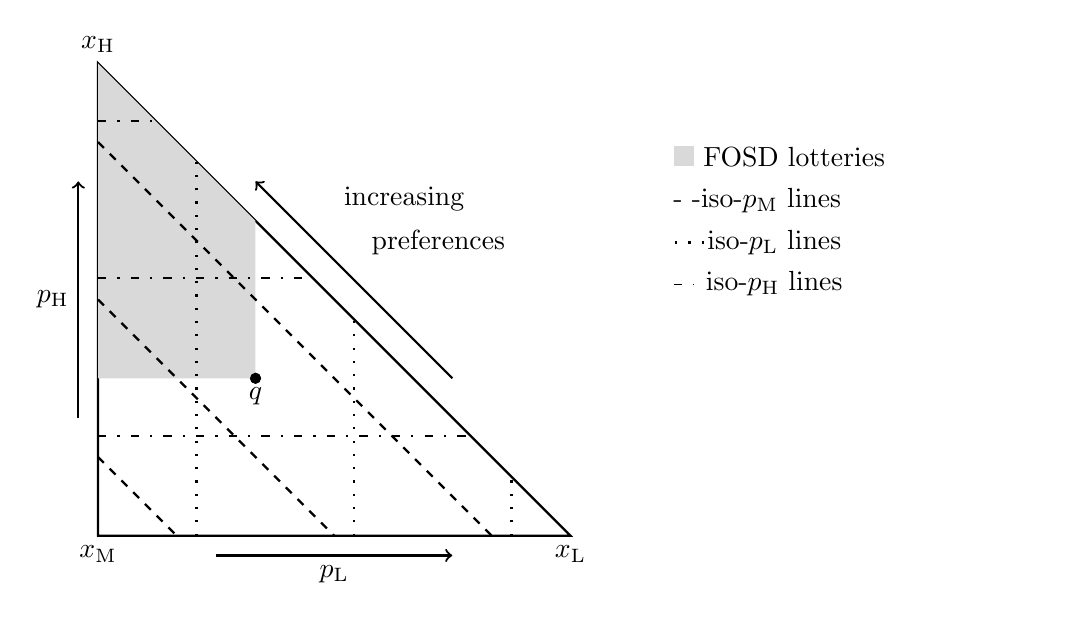
\begin{tikzpicture}
%M-M triangle
\draw[thick] (0,0) node[align=left, below] {$x_{\midd}$}
-- (0, 6) node[align=left, above] {$x_{\hi}$}
-- (6, 0) node[align=left, below] {$x_{\low}$}
--cycle;

%Improving p_{\hi}
\draw[->,thick] (-.25,1.5) -- (-.25,4.5);
\draw (-.25,3) node[align=left, left] {$p_{\hi}$};
%Improving p_{\low}
\draw[->,thick] (1.5,-.25) -- (4.5,-.25);
\draw (3,-.25) node[align=left, below] {$p_{\low}$};


%Improving Preferences
\draw[->,thick] (4.5,2) -- (2,4.5);
\draw (3,4) node[align=left, right] {increasing\\[.1em] \quad preferences};


\fill[black] (2,2) circle[radius=2pt];
\draw (2,2) node[align=left, below] {$q$};


%Better than lotteries
\draw[draw opacity=0, fill=gray!30]
(2,2)
-- (2,4)
-- (0,6)
-- (0,2)
--cycle;
\fill[black] (2,2) circle[radius=2pt];

%Iso p_{\midd}
\draw[thick, dashed] (0,1) -- (1,0);
\draw[thick, dashed] (0,3) -- (3,0);
\draw[thick, dashed] (0,5) -- (5,0);

%Iso p_{\low}
\draw[thick, loosely dotted] (1.25,0) -- (1.25,4.75);
\draw[thick, loosely dotted] (3.25,0) -- (3.25,2.75);
\draw[thick, loosely dotted] (5.25,0) -- (5.25,.75);

%Iso p_{\low}
\draw[thick, loosely dashdotted] (0,1.27) -- (4.73,1.27);
\draw[thick, loosely dashdotted] (0,3.27) -- (2.73,3.27);
\draw[thick, loosely dashdotted] (0,5.27) -- ( .73, 5.27);

%Legend
\draw[xshift=12cm, yshift=4cm] node [ left,text width=13em]
{
\tikz\draw[draw opacity=0,fill=gray!30] (0,0) rectangle (.25,.25); FOSD lotteries\\
- -iso-$p_{\midd}$ lines\\
\hwplotA  iso-$p_{\low}$ lines\\
\hwplotB  iso-$p_{\hi}$ lines
};
\end{tikzpicture}
        \caption{Marschak-Machina Triangle}\label{fig:MM}
\end{figure}

We now describe some features of the MM triangle from Figure~\ref{fig:MM}. First, the dashed lines in Figure~\ref{fig:MM} all have the same probability of receiving the middle prize. We refer to the dashed lines as iso-$p_{\midd}$ lines. As the dashed lines move northeast, the level of $p_{\midd}$ decreases. Similarly, the dotted lines all have the same probability of receiving the low price, so we refer to these as iso-$p_{\low}$ lines. As the dotted lines move east, the probability of receiving the low prize increases. Finally, the dash-dotted lines have the same probability of $p_{\hi}$ so we refer to these as iso-$p_{\hi}$ lines. As these lines move north the probability of receiving the high prize increases.

The one property we assume for risk preferences is first order stochastic dominance (FOSD). The lottery $p'=(p_{\low}',p_{\midd}', p_{\hi}')$ first order stochastic dominates the lottery $p=(p_{\low},p_{\midd}, p_{\hi})$ when $p'_{\hi}\ge p_{\hi}$ and $p'_{\hi}+p'_{\midd} \ge p_{\hi}+p_{\midd}$ with one inequality strict. For example, the lotteries that FOSD the lottery $q$ in Figure~\ref{fig:MM} are those that lie to the west (less $p_{\low}$ more $p_{\midd}$) or north (less $p_\midd$ more $p_\hi$) of $q$. Since preferences respect first order stochastic dominance, the lotteries to the northwest are more preferred which is indicated with the arrow labeled ``increasing preferences" in Figure~\ref{fig:MM}.

For the experiment, we elicit individual choices from convex budget sets. Importantly, a convex budget allows individuals to choose lotteries that are a mixture of the ``corners" of the budget set. This design feature is essential since many theories of non-expected utility allow an individual to prefer mixtures of lotteries from convex budgets.\footnote{One notable class that does not allow mixtures except for the case of indifference is the betweenness class of preferences \cite{Dekel/1986}.} In contrast, if an individual has expected utility preferences, then they will almost always choose lotteries on the boundary of the MM triangle and cannot choose mixtures from budgets with two different slopes. We argue it is important to elicit a preference for mixing using convex budget sets since an individual may ``convexify" discrete choice problems by randomizing among the lotteries to mimic their most preferred lottery from a convex budget set.

We introduce some terminology to describe how budget sets are constructed. Each budget in the experiment is generated by a line connecting two lotteries that lie on the boundary of the MM triangle. In particular, we choose an \emph{extreme lottery} and a \emph{numeraire lottery} to generate each budget line. The \emph{extreme lottery} is denoted $p^{\srd}$ and places probability exclusively on the extreme high and low prizes. The \emph{numeraire lottery} is denoted $p^{\edw}$, places some probability on the middle prize and is on the boundary of the MM triangle, serves as a reference lottery that budget lines pivot around, and allows us to examine changes in the relative price for a given numeraire lottery. A series of example budgets that pivot around a numeraire lottery are shown in Figure~\ref{fig:priceOff}.

\begin{figure}[H]
	\centering
	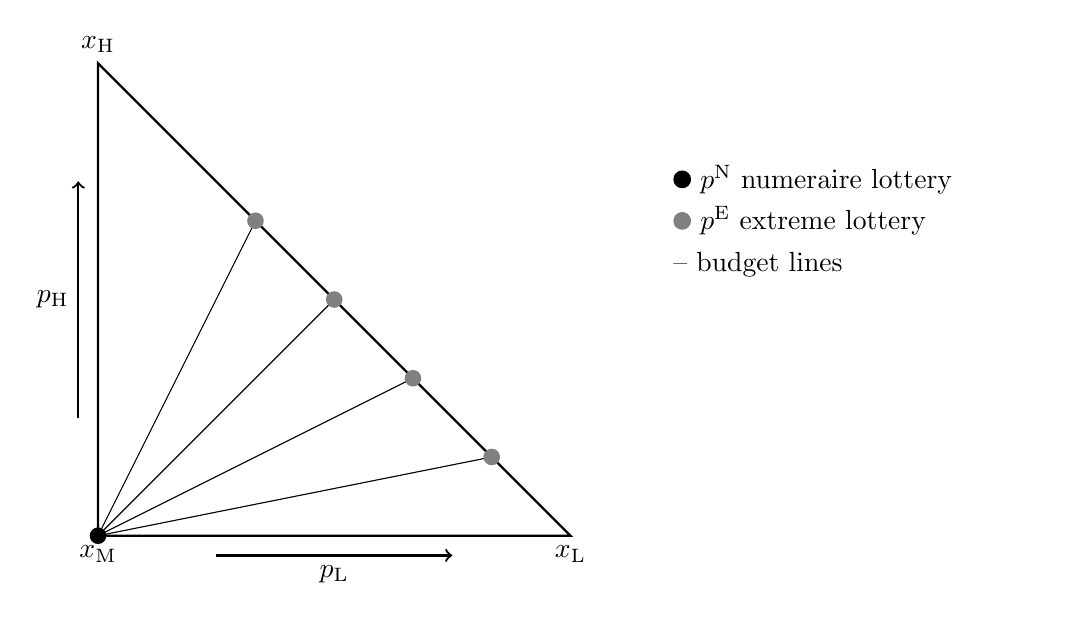
\begin{tikzpicture}
	%M-M triangle
	\draw[thick] (0,0) node[align=left,   below] {$x_{\midd}$}
		-- (0, 6) node[align=left,   above] {$x_{\hi}$}
		-- (6, 0) node[align=left,   below] {$x_{\low}$}
		--cycle;

	%Improving p_{\hi}
	\draw[->,thick] (-.25,1.5) -- (-.25,4.5);
	\draw (-.25,3) node[align=left, left] {$p_{\hi}$};

	%Improving p_{\low}
	\draw[->,thick] (1.5,-.25) -- (4.5,-.25);
	\draw (3,-.25) node[align=left, below] {$p_{\low}$};

	%Draw three budgets
	%% Lines
	\draw (0,0)--(5,1);
	\draw (0,0)--(4,2);
	\draw (0,0)--(3,3);
	\draw (0,0)--(2,4);

	%% p^{\edw}
 	\fill[black] (0,0)  circle[radius=3pt];
	
	%% Second p^{srd}
	\fill[gray] (4,2)  circle[radius=3pt];
	\fill[gray] (5,1)  circle[radius=3pt];
	\fill[gray] (3,3) circle[radius=3pt];
	\fill[gray] (2,4) circle[radius=3pt];

	%Legend
	\draw[xshift=12cm, yshift=4cm] node [ left,text width=13em]
   	 {
	\tikz\draw[black,fill=black] (0,0) circle (3pt); $p^{\edw}$ numeraire lottery \\
	\tikz\draw[gray, fill=gray] (0,0) circle (3pt); $p^{\srd}$ extreme lottery\\
	-- budget lines 
  	  };
	\end{tikzpicture}
	\caption{``Price" Variation}
        	\label{fig:priceOff}
        	\raggedright
        	            \iffalse
        	            \footnotesize{ This figure illustrates the "price" changes. As we move across the budgets, from right to left, the slope ("price") increases. This slope measures how much the likelihood of the high outcome increases with respect to likelihood of the low outcome as we decrease the likelihood of the middle outcome. Higher "prices" imply the ratio
        	            of likelihood between high and low outcomes is more desirable in terms of first order stochastic dominance.} 
        	            \fi
\end{figure}

The reason we examine a series of budgets that pivot around a numeraire lottery is to examine a ``demand" curve for the numeraire lottery. To see this, note that for a fixed numeraire lottery, $p^{\edw}$, the slope of a budget line is essentially a relative price for the numeraire lottery. To better understand the analogy between the slope and a ``price" for the numeraire lottery, note that as the probability of receiving the high prize of the extreme lottery increases, the extreme lottery becomes more attractive, and the slope of the budget line increases. Thus, we say the relative price ($r$) for the numeraire lottery is given by
 \[ r = \frac{p_{\hi}^{\srd}-p_{\hi}^{\edw}}{p_{\low}^{\srd}-p_{\low}^{\edw}}.\]
We later examine how the aggregate demands for the numeraire lotteries vary with the relative prices. We note that the interpretation of $r$ as a relative price of the numeraire lottery is a feature of linear budget sets and does not depend on preferences.

\section{Experimental Design}\label{sec:design}
%%%%%%%%%%%%%%%%%%%%%%%%%%%%%%%%%%%%%%%%%%%%%%%%%%%%%%%%%

In this section, we describe the details of our experimental design. Subjects completed 85 different choice tasks in the experiment. For each choice task, budgets consist of lotteries over the monetary prizes $x_{\low}= \$2$, $x_{\midd}= \$10$, and $x_{\hi}=\$30$.\footnote{These payments are the same order of magnitude as other studies of risk (see for example \cite{camerer/harless/1994}, \cite{hey/orme/1994},  \cite{sprenger/2015}, among others). Our key design choice was to operate in the domain of only gains to not involve loss aversion.}  In each task, a subject selects a preferred lottery from a given budget set. There are two types of choice tasks: convex choice tasks and repeated discrete choice tasks. The subjects first faced 79 convex choice tasks from linear budget sets that consist of convex combinations of a numeraire lottery ($p^{\edw}$) and an extreme lottery ($p^{\srd}$) in a random order. The remaining six tasks were discrete choice tasks where a subject could choose either the numeraire lottery ($p^{\edw}$) or the extreme lottery ($p^{\srd}$). In particular, these six tasks were three repeated discrete choices from two distinct choice tasks.

One hundred and forty-four undergraduates from UC San Diego participated in this study. Six sessions were conducted from January 22-23 in 2018. The tasks were conducted on internet-enabled laptops through a web browser and the design was coded in oTree \citep{otree/2016}. The experiment was separated into three sections: examples, convex choice tasks (79 tasks), and discrete choice tasks (6 tasks). Instructions were provided to each subject before the session and read aloud by the experimenter. The full set of instructions can be found in Appendix~\ref{app:inst}. Subjects were paid according to one randomly chosen decision in the experiment to ensure truthful revelation of preferences. We use a physical randomization device to resolve all uncertainty. Further details on how the randomization was carried out and why we chose to pay one decision are in Appendix~\ref{app:payone}. There was a \$10 show-up fee. On average subjects earned \$23.15 in total. Subjects spent an average of 15.8 seconds per convex choice task and 12.3 seconds per binary choice task.

\subsection{Convex Choice Tasks}\label{sec:convchoices}
The first set of choice tasks have convex budgets generated from a numeraire lottery and an extreme lottery as in Figure~\ref{fig:priceOff}. In more detail, an individual could choose any distribution from 
\begin{equation}\label{eq:alpha}
p(\alpha)=\frac{\alpha}{100}  p^{\edw} + \frac{100-\alpha}{100} p^{\srd} \end{equation}
where $\alpha \in \{0,\ldots,100\}$. Thus, a choice of the extreme lottery, $p^{\srd}$, corresponds to $\alpha=0$, a choice of the numeraire lottery, $p^{\edw}$, corresponds to $\alpha=100$, and a choice of a mixture corresponds to $\alpha \in \{1,\ldots, 99\}$. The fineness of the convexification of the budget mimics that of other experiments (e.g. \cite{choi/etal/2007}). 

While convex budgets in the MM triangle are easy for economists to understand, we use a more familiar representation of probabilities to elicit choices from subjects. In particular, we build on the interface pioneered by \cite{sopher/narramore/2000} that uses a pie chart to display the simple lottery that corresponds to a given $\alpha$ mixture. An example of the pie chart and the choice interface is shown in Figure~\ref{fig:Example}. For each choice task, the prizes $x_{\low}= \$2$, $x_{\midd}= \$10$, and $x_{\hi}=\$30$ are displayed at the top of the interface and color-coded to match the appropriate region on the pie chart. As the subject interacts with the slide-rule, the pie chart updates to reflect the lottery induced by mixing a numeraire and extreme lottery for a given $\alpha$ mixture. Our interface was chosen because it is intuitive for representing three outcome lotteries, makes the trade-off between the numeraire and extreme lottery salient, and has already been used in the experimental literature \citep{ sopher/narramore/2000, karni/etal/2008}. Moreover, \cite{simkin1987information} find that pie charts are an efficient mechanism for emphasizing the likelihood of each outcome relative to the whole.

\begin{figure}[h]
    \centering
    \fbox{ \includegraphics[width=.7\textwidth, angle=-90]{figs/task_g.pdf}}
        \caption{Example of a Task}\label{fig:Example}
        \raggedright
\end{figure}
\newpage
We now discuss some important design features of the interface. At the start of each task, the pie chart is not displayed until the subject interacts with the slide rule and the slide rule is positioned at $\alpha=50$. Since the pie chart is not displayed, we believe framing effects from the slide rule at $\alpha=50$ should be mitigated since a subject needs to interact with the slide rule to see the lottery. There are also advantages to keeping the slide rule initialized at a fixed position. First, we do not introduce idiosyncratic noise in the choices by using a random starting point on all tasks. We were also concerned that the random starting point would induce framing effects for the repeated discrete choice tasks since subjects could be drawn to the lottery that is closest to the random starting point. Finally, the choice of a fixed starting point allows us to examine experimenter demand effects since we can compare the behavior of subjects to behavior that simulates possible demand effects. In particular, we compare the choices of subjects in the experiment to noisy choices around the midpoint of $\alpha=50$. One final difference of the design from \cite{sopher/narramore/2000} is that subjects cannot proceed to the next choice task until they interact with the slider and re-affirm their choice by typing it in the box below ``Verify". This design feature helps to ensure that subjects are expressing a preference for whatever $\alpha$ mixture they select.

Throughout the experiment, the location of the extreme lottery, $p^{\srd}$, is fixed at $\alpha=0$ and the location of the numeraire lottery, $p^{\edw}$, is fixed at $\alpha=100$. We made this design choice so that individuals would be able to quickly understand the structure of the experiment. Since it is easy to discern extreme lotteries from numeraire lotteries, we believe this makes it easier for individuals to make choices consistent with no mixing behavior. Lastly, we display the lottery from the mixture $\frac{\alpha}{100}  p^{\edw} + \frac{100-\alpha}{100} p^{\srd}$ as a simple one-stage lottery. This design feature eliminates any errors that result when individuals fail to reduce compound lotteries.

Next, we describe the budget sets that individuals face in the experiment. We used eight different numeraire lotteries to generate convex budgets. We refer to these lotteries in the text as N1-N8, where the lotteries take the values in Table~\ref{tab:edw}.  The reference lotteries N1-N8 are ordered by first order stochastic dominance so that when $k>j$, the lottery $p^{\edw k}$ first order stochastic dominates $p^{\edw j}$.\footnote{We focus on numeraire lotteries on the high/middle axis to direct power where the expected value is high enough to have payoffs which are nontrivial.}

\begin{table}[h]
\small
\centering
\begin{tabular}{l | llllllll}
\hline
 & N1 & N2 & N3 & N4 & N5 & N6 & N7 & N8\\
\hline
$p_{\$2}$ & .50 & 0 & 0 & 0 & 0 & 0 & 0 & 0 \\
$p_{\$10}$ & .50 & 1 & .90 & .75 & .60 & .45 & .30 & .15\\
$p_{\$30}$ & 0 & 0 & .10 & .25 & .40 & .55 & .70 & .85 \\
\hline
\end{tabular}
\caption{Reference Lotteries}\label{tab:edw}
\end{table}

We summarize all budgets for the convex choice tasks in the MM triangle in Figure~\ref{fig:budgets}.\footnote{We piloted sessions where individuals were restricted to choose mixtures on the interior of the simplex and found individuals made choices at the boundary. For this reason, we allowed the choices to go to the boundary. The results are qualitatively similar.} Recall that the budget lines are designed to pivot around the numeraire lotteries to examine how mixing behavior varies with the relative price of a numeraire lottery. All subjects face the same set of 79 budgets, but the order of the budgets is randomized for each subject. The budget lines all have strictly positive slopes in the MM triangle so that no lotteries in the budget are ordered by first order stochastic dominance.\footnote{There were more budgets for questions when the numeraire is of intermediate value to increase the potential violations of utility maximization in the revealed preference analysis described in Section~\ref{sec:revealed}.}  This feature allows us to focus on violations resulting from mixing behavior without worrying about subjects satisfying the FOSD property within a budget. This feature is similar to other revealed preference experiments that restrict subjects from expressing satiation \citep{andreoni2002giving, choi/etal/2007, andreoni2011uncertainty, andreoni2012estimating, Andreoni/Sprenger/RiskTime}. 

\begin{figure}[H]
	\centering
	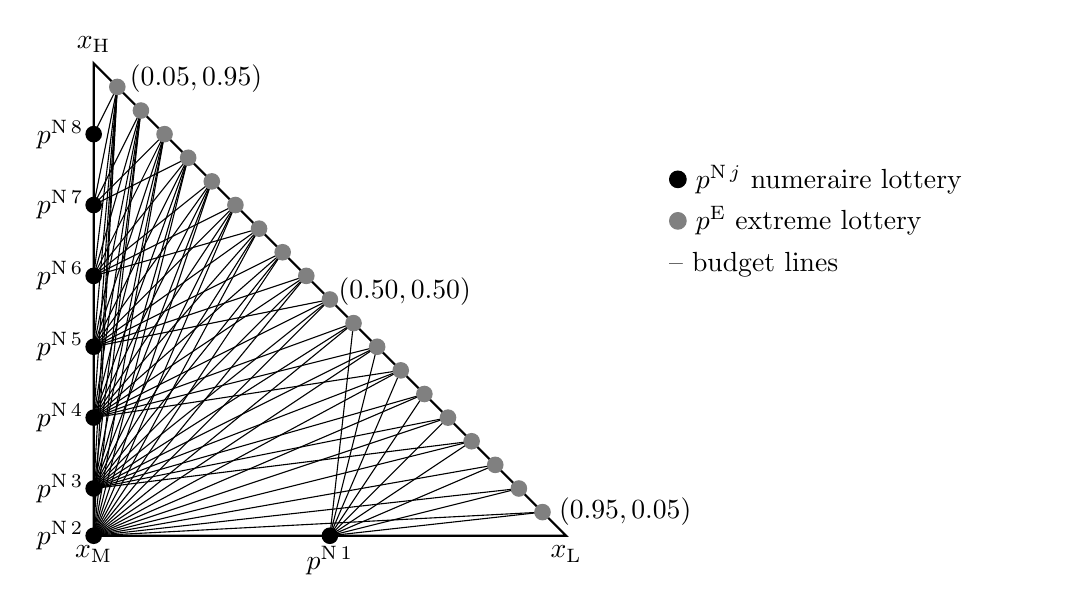
\begin{tikzpicture}[scale=1]
	%Non-STD M-M triangle
	\draw[thick] (0,0) node[align=left,   below] {$x_{\midd} $}  %changed low to L,hi to H and Midd to M 
		-- (0, 6) node[align=left,   above] {$x_{\hi} $}
		-- (6, 0) node[align=left,   below] {$x_{\low} $}
		--cycle;
         
         \draw[thick] (6*.5,0)  node[align=left, below] {$p^{\edw 1}$}; %Endowment 1
	\draw[thick] (0,0)  node[align=left, left] {$p^{\edw 2}$}; %Endowment 2
 	\draw[thick] (0,6*.1)  node[align=left, left] {$p^{\edw 3}$}; %Endowment 3
 	\draw[thick] (0,6*.25)  node[align=left, left] {$p^{\edw 4}$}; %Endowment 4
 	\draw[thick] (0,6*.4)  node[align=left, left] {$p^{\edw 5}$}; %Endowment 5
 	\draw[thick] (0,6*.55)  node[align=left, left] {$p^{\edw 6}$}; %Endowment 6
 	\draw[thick] (0,6*.7)  node[align=left, left] {$p^{\edw 7}$}; %Endowment 7
 	\draw[thick] (0,6*.85)  node[align=left, left] {$p^{\edw 8}$}; %Endowment 8
         
         
         \draw[thick,black] (6*.95+.65+.4,6*.05-.3) node[align=right, above] {$(0.95,0.05)$};
         \draw[thick,black] (6*.5+.65+.3,6*.5-.2) node[align=right, above] {$(0.50,0.50)$};
         \draw[thick,black] (6*.05+.65+.35,6*.95-.2) node[align=right, above] {$(0.05,0.95)$};
 
 	%Endowment 1: Budgets x 9
	\draw[black] (6*.5,0)  -- (6*.95,6-6*.95) ;
	\draw[black] (6*.5,0)  -- (6*.90,6-6*.90) ;
	\draw[black] (6*.5,0)  -- (6*.85,6-6*.85) ;
	\draw[black] (6*.5,0)  -- (6*.80,6-6*.80) ;
	\draw[black] (6*.5,0)  -- (6*.75,6-6*.75) ;
	\draw[black] (6*.5,0)  -- (6*.70,6-6*.70) ;
	\draw[black] (6*.5,0)  -- (6*.65,6-6*.65) ;
	\draw[black] (6*.5,0)  -- (6*.60,6-6*.60) ;
	\draw[black] (6*.5,0)  -- (6*.55,6-6*.55) ;
	%Endowment 2: Budgets x 19
	\draw[black] (0,0)  -- (6*.95,6-6*.95) ;
	\draw[black] (0,0)  -- (6*.90,6-6*.90) ;
	\draw[black] (0,0)  -- (6*.85,6-6*.85) ;
	\draw[black] (0,0)  -- (6*.80,6-6*.80) ;
	\draw[black] (0,0)  -- (6*.75,6-6*.75) ;
	\draw[black] (0,0)  -- (6*.70,6-6*.70) ;
	\draw[black] (0,0)  -- (6*.65,6-6*.65) ;
	\draw[black] (0,0)  -- (6*.60,6-6*.60) ;
	\draw[black] (0,0)  -- (6*.55,6-6*.55) ;
	\draw[black] (0,0)  -- (6*.50,6-6*.50) ;
	\draw[black] (0,0)  -- (6*.45,6-6*.45) ;
	\draw[black] (0,0)  -- (6*.40,6-6*.40) ;
	\draw[black] (0,0)  -- (6*.35,6-6*.35) ;
	\draw[black] (0,0)  -- (6*.30,6-6*.30) ;
	\draw[black] (0,0)  -- (6*.25,6-6*.25) ;
	\draw[black] (0,0)  -- (6*.20,6-6*.20) ;
	\draw[black] (0,0)  -- (6*.15,6-6*.15) ;
	\draw[black] (0,0)  -- (6*.10,6-6*.10) ;
	\draw[black] (0,0)  -- (6*.05,6-6*.05) ;
	%Endowment 3: Budgets x 16
	\draw[black] (0,6*.1)  -- (6*.80,6-6*.80) ;
	\draw[black] (0,6*.1)  -- (6*.75,6-6*.75) ;
	\draw[black] (0,6*.1)  -- (6*.70,6-6*.70) ;
	\draw[black] (0,6*.1)  -- (6*.65,6-6*.65) ;
	\draw[black] (0,6*.1)  -- (6*.60,6-6*.60) ;
	\draw[black] (0,6*.1)  -- (6*.55,6-6*.55) ;
	\draw[black] (0,6*.1)  -- (6*.50,6-6*.50) ;
	\draw[black] (0,6*.1)  -- (6*.45,6-6*.45) ;
	\draw[black] (0,6*.1)  -- (6*.40,6-6*.40) ;
	\draw[black] (0,6*.1)  -- (6*.35,6-6*.35) ;
	\draw[black] (0,6*.1)  -- (6*.30,6-6*.30) ;
	\draw[black] (0,6*.1)  -- (6*.25,6-6*.25) ;
	\draw[black] (0,6*.1)  -- (6*.20,6-6*.20) ;
	\draw[black] (0,6*.1)  -- (6*.15,6-6*.15) ;
	\draw[black] (0,6*.1)  -- (6*.10,6-6*.10) ;
	\draw[black] (0,6*.1)  -- (6*.05,6-6*.05) ;
	%Endowment 4: Budgets x 13
	\draw[black] (0,6*.25)  -- (6*.65,6-6*.65) ;
	\draw[black] (0,6*.25)  -- (6*.60,6-6*.60) ;
	\draw[black] (0,6*.25)  -- (6*.55,6-6*.55) ;
	\draw[black] (0,6*.25)  -- (6*.50,6-6*.50) ;
	\draw[black] (0,6*.25)  -- (6*.45,6-6*.45) ;
	\draw[black] (0,6*.25)  -- (6*.40,6-6*.40) ;
	\draw[black] (0,6*.25)  -- (6*.35,6-6*.35) ;
	\draw[black] (0,6*.25)  -- (6*.30,6-6*.30) ;
	\draw[black] (0,6*.25)  -- (6*.25,6-6*.25) ;
	\draw[black] (0,6*.25)  -- (6*.20,6-6*.20) ;
	\draw[black] (0,6*.25)  -- (6*.15,6-6*.15) ;
	\draw[black] (0,6*.25)  -- (6*.10,6-6*.10) ;
	\draw[black] (0,6*.25)  -- (6*.05,6-6*.05) ;
	%Endowment 5: Budgets x 10
	\draw[black] (0,6*.4)  -- (6*.50,6-6*.50) ;
	\draw[black] (0,6*.4)  -- (6*.45,6-6*.45) ;
	\draw[black] (0,6*.4)  -- (6*.40,6-6*.40) ;
	\draw[black] (0,6*.4)  -- (6*.35,6-6*.35) ;
	\draw[black] (0,6*.4)  -- (6*.30,6-6*.30) ;
	\draw[black] (0,6*.4)  -- (6*.25,6-6*.25) ;
	\draw[black] (0,6*.4)  -- (6*.20,6-6*.20) ;
	\draw[black] (0,6*.4)  -- (6*.15,6-6*.15) ;
	\draw[black] (0,6*.4)  -- (6*.10,6-6*.10) ;
	\draw[black] (0,6*.4)  -- (6*.05,6-6*.05) ;
	%Endowment 6: Budgets x 7
	\draw[black] (0,6*.55)  -- (6*.35,6-6*.35) ;
	\draw[black] (0,6*.55)  -- (6*.30,6-6*.30) ;
	\draw[black] (0,6*.55)  -- (6*.25,6-6*.25) ;
	\draw[black] (0,6*.55)  -- (6*.20,6-6*.20) ;
	\draw[black] (0,6*.55)  -- (6*.15,6-6*.15) ;
	\draw[black] (0,6*.55)  -- (6*.10,6-6*.10) ;
	\draw[black] (0,6*.55)  -- (6*.05,6-6*.05) ;
	%Endowment 7: Budgets x 4
	\draw[black] (0,6*.7)  -- (6*.20,6-6*.20) ;
	\draw[black] (0,6*.7)  -- (6*.15,6-6*.15) ;
	\draw[black] (0,6*.7)  -- (6*.10,6-6*.10) ;
	\draw[black] (0,6*.7)  -- (6*.05,6-6*.05) ;
	%Endowment 8: Budgets x 1
	\draw[black] (0,6*.85)  -- (6*.05,6-6*.05) ;
	%Endowments
	\fill[black] (6*.5,0)  circle[radius=3pt]; %Endowment 1
	\fill[black] (0,0)  circle[radius=3pt]; %Endowment 2
 	\fill[black] (0,6*.1)  circle[radius=3pt]; %Endowment 3
 	\fill[black] (0,6*.25)  circle[radius=3pt]; %Endowment 4
 	\fill[black] (0,6*.4)  circle[radius=3pt]; %Endowment 5
 	\fill[black] (0,6*.55)  circle[radius=3pt]; %Endowment 6
 	\fill[black] (0,6*.7)  circle[radius=3pt]; %Endowment 7
 	\fill[black] (0,6*.85)  circle[radius=3pt]; %Endowment 8
	%Spreads
	\fill[gray] (6*.95,6-6*.95) circle[radius=3pt];
	\fill[gray] (6*.90,6-6*.90) circle[radius=3pt];
	\fill[gray] (6*.85,6-6*.85) circle[radius=3pt];
	\fill[gray] (6*.80,6-6*.80) circle[radius=3pt];
	\fill[gray] (6*.75,6-6*.75) circle[radius=3pt];
	\fill[gray] (6*.70,6-6*.70) circle[radius=3pt];
	\fill[gray] (6*.65,6-6*.65) circle[radius=3pt];
	\fill[gray] (6*.60,6-6*.60) circle[radius=3pt];
	\fill[gray] (6*.55,6-6*.55) circle[radius=3pt];
	\fill[gray] (6*.50,6-6*.50) circle[radius=3pt];
	\fill[gray] (6*.45,6-6*.45) circle[radius=3pt];
	\fill[gray] (6*.40,6-6*.40) circle[radius=3pt];
	\fill[gray] (6*.35,6-6*.35) circle[radius=3pt];
	\fill[gray] (6*.30,6-6*.30) circle[radius=3pt];
	\fill[gray] (6*.25,6-6*.25) circle[radius=3pt];
	\fill[gray] (6*.20,6-6*.20) circle[radius=3pt];
	\fill[gray] (6*.15,6-6*.15) circle[radius=3pt];
	\fill[gray] (6*.10,6-6*.10) circle[radius=3pt];
	\fill[gray] (6*.05,6-6*.05) circle[radius=3pt];
	%Legend
	\draw[xshift=12cm, yshift=4cm] node [ left,text width=13em]
   	 {
	\tikz\draw[black,fill=black] (0,0) circle (3pt); $p^{\edw j}$ numeraire lottery \\
	\tikz\draw[gray,fill=gray] (0,0) circle (3pt); $p^{\srd }$ extreme lottery\\
	-- budget lines
  	  };
	\end{tikzpicture}
	\caption{Budget Lines in the Marshack-Machina Triangle}\label{fig:budgets}
	\raggedright
	  \footnotesize{\textbf{Notes:} This figure sketches all the budgets that subjects face during the experiment in the Machina Marchak triangle. Subjects never saw this visual representation.}
\end{figure}

\subsection{Discrete Choice Tasks}
Here we describe the six binary discrete choice tasks each subject faces. These tasks were completed after all seventy-nine convex choice tasks and use the same interface described above. The one difference is that $\alpha$ could only take the values of zero or one hundred when moved from the initial position. Thus, a subject could only choose either a numeraire lottery or an extreme lottery. In particular, we examine the binary choice tasks $D_1 = \{(0,0.9,0.1),  (0.65,0,0.35) \}$ and $D_2 = \{ (0.5,0.5,0), (0.95,0,0.05)\}$ where the first lottery is a numeraire lottery and the second is an extreme lottery. The numeraire lottery in D1 is N3, while the numeraire lottery in D2 is N1. Each subject first faced three repeated discrete choice tasks from D1, then faced three repeated discrete choice tasks from D2. For each budget, the subject knew before choosing that they would face each budget set three consecutive times with each repetition appearing on a different screen. This follows the experimental design in \cite{Agranov/Ortoleva/2017} to prevent the realization of several random shocks to elicit a preference for randomization.

\begin{figure}[H]
	\centering
	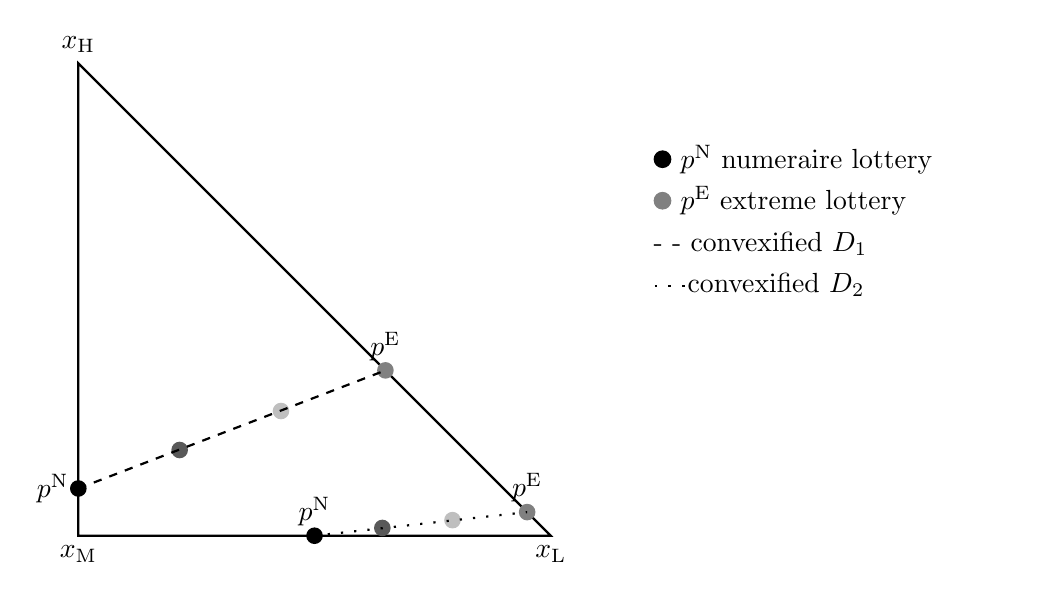
\begin{tikzpicture}
	%Non-STD M-M triangle
	\draw[thick] (0,0) node[align=left,   below] {$x_{\midd} $}
		-- (0, 6) node[align=left,   above] {$x_\hi$}
		-- (6, 0) node[align=left,   below] {$x_\low$}
		--cycle;

	
	%% D1 Choices
 	\fill[black] (0,.1*6)  circle[radius=3pt];
 	\draw [black] (0,.1*6) node[align=left, left] {$p^{\edw}$};
	\fill[gray] (6*.65,6*.35)  circle[radius=3pt];
	\draw [black] (6*.65,6*.35) node[align=right,above] {$p^{\srd}$};
	\fill[black!65] (.33*6*.65 , .33*6*.35+.66*.6 )  circle[radius=3pt];
	\fill[gray!50] (.66*6*.65 , .66*6*.35+.33*.6 )  circle[radius=3pt];
	
	%% D2 Choices
	\fill[black] (3,0)  circle[radius=3pt];
 	\draw [black] (3,0) node[align=left, above] {$p^{\edw}$};
	\fill[gray] (6*.95,6*.05)  circle[radius=3pt];
	\draw [black] (6*.95,6*.05) node[align=left, above] {$p^{\srd}$};
	\fill[black!65] (.33*6*.95+.66*3 , .33*6*.05 )  circle[radius=3pt];
	\fill[gray!50] (.66*6*.95+.33*3 , .66*6*.05 )  circle[radius=3pt];
	\draw (5,5) node[align=left, above] {};
	
	
	%% Indifference between D1
	\draw[thick, dashed] (0,0.6) -- (6*.65,6*.35);
	%% Indifference between D2
	\draw[thick, loosely dotted] (3,0) -- (6*.95,6*.05);
	
	
		%Legend
	\draw[xshift=12cm, yshift=4cm] node [ left,text width=13em]
   	 {
	\tikz\draw[black,fill=black] (0,0) circle (3pt); $p^{\edw}$ numeraire lottery \\
	\tikz\draw[gray,fill=gray] (0,0) circle (3pt); $p^{\srd}$ extreme lottery\\
	- -  convexified $D_1$\\
	\hwplotA convexified $D_2$
  	  };
	\end{tikzpicture}
	\caption{Discrete-Choice Tasks and Implied Mixtures}
	 \label{fig:bin}
	 \raggedright
	  \footnotesize{\textbf{Notes:} Subjects only choose between the pairs of the numeraire and the extreme lotteries. The discrete task was repeated three times so that the shaded points represent implied mixtures that could be chosen.}
\end{figure}

Each discrete choice budget is linked with a convex choice task in the first part of the experiment. While the convex choice tasks are designed to elicit information about whether an individual prefers mixtures of lotteries, these choice tasks are designed to see whether mixing behavior is related to behavior from repeated discrete choices. In particular, if this behavior is related, then individuals should have repeated discrete choices that mimic the choice from the convex budget. The implied mixtures a subject could choose from three discrete choice tasks are shown in Figure~\ref{fig:bin}. We later show that choices in the two domains are positively correlated. We take this as evidence that an individual's non-linear risk preferences and preference for randomization are linked.

We note that the relative price, $r$, of the numeraire lottery in both environments favors the numeraire lottery since $r_{D_1} \approx .38$ and $r_{D_2} \approx .11$ both of which are less than one. If there is little mixing, then we should be better able to detect whether there is any correlation between behavior from the two elicitation methods since boundary choices are intuitively easier for individuals to make. Thus, one could interpret the relationship we find between behavior in the convex choice task and repeated discrete choice task as an upper-bound on the correlation between tasks. 

%%%%%%%%%%%%%%%%%%%%%%%
\section{Main Results}\label{sec:results}
%%%%%%%%%%%%%%%%%%%%%%%

In this section, we present the main results of the experiment. We re-state our two main hypotheses below.

\begin{hypothesis1} Many individuals will choose mixtures, and behavior will be inconsistent with expected utility predictions.  
\end{hypothesis1}
\begin{hypothesis2} The decisions from the convex choice tasks and the repeated discrete choice tasks will be positively correlated with one another.   
\end{hypothesis2}

We briefly summarize the main results and provide additional detail in the following subsections. We find support for Hypothesis~\ref{hyp:mixing} since 136/144 subjects mix at least once, and only 1/144 subject can be described by expected utility. We also find support for Hypothesis~\ref{hyp:discrete}. In particular, we find that most of the mixture lotteries implied by the three repeated discrete choices are within one choice from the behavior in the convex choice task. We also find that behavior from the convex and repeated discrete choice tasks are positively correlated. These results suggest that an individual's preference for mixtures is related to behavior in the repeated discrete choice task.

\subsection{Mixing Behavior from Convex Choice Tasks}

For the convex choice tasks, we say a subject mixes in a convex choice task when $\alpha \in \{1, 2, \ldots, 99\}$.\footnote{Results are robust to the threshold used to define ``mixing."  For example, when we say a subject mixes in a task for $\alpha \in \{ 0+c, \ldots, 100-c \}$ results are qualitatively similar for $c=2$ or $c=5$. See Appendix~\ref{app:AltMix} for details.} Result~\ref{res:mixing} collects the main evidence that supports Hypothesis~\ref{hyp:mixing}.

\begin{result}\label{res:mixing} Mixing behavior is common in the convex choice tasks.
			\begin{enumerate}[(a)]
				\item 136/144 (94.4\%) subjects mix at least once.
				\item 44.6\% of all choices exhibit a preference for mixing.
				\item 1/144 subjects has choices that can be described by expected utility.
			\end{enumerate}
\end{result}

First, we show the histogram of how often subjects chose a mixture in Figure~\ref{fig:histMix}. We find that 56/144 (38.9\%) subjects mix in over thirty-nine convex choice tasks (over half of all choice tasks). There are also 16/144 (11.1\%) individuals choosing to mix in seventy or more convex choice tasks. We take these results as evidence against expected utility since this theory predicts (almost) no mixing. Moreover, we find 131/144 (91\%) subjects chose mixtures from budgets with different slopes which is a quick heuristic that refutes expected utility. In fact, expected utility is satisfied by only one subject.

% Mixtures
\begin{figure}[H]
  \centering
        \includegraphics[width=.4\textwidth]{figs/MixHist.png}
       \caption{Histogram of Mixing Behavior}\label{fig:histMix}
       \raggedright
\end{figure}

Next, we show the percentage of choices for the numeraire lottery, extreme lottery, and mixtures for budgets generated from different numeraire lotteries in Table~\ref{tab:endowMix}. We find that the most mixing occurs in convex choice tasks with numeraire lottery N3, which has a 90\% chance of \$10 and a 10\% chance of \$30 (or $(0,0.90,0.10)$). The least mixing occurs for the convex choice task for N8 which likely occurs from the single relative price used at these budgets. We do not have the same prices at each numeraire lottery since we were trying to maximize the ability to compare individual choices to certain benchmark behavior in a later revealed preference analysis. Thus, other than the fact that mixing occurs for all numeraire lotteries, we encourage caution in drawing conclusion from the comparative static with regards to mixing and first order stochastic dominating numeraire lotteries.

\begin{table}[H] 
\small
\centering  
\begin{tabular}{l |llllllll|l} 
\hline
& N1 & N2 & N3 & N4 & N5 & N6 & N7 & N8 & Total\\
\hline
Mix & 33\% & 45\% & 51\% & 50\% & 45\% & 42\% & 30\% & 18\% & 44\% \\
Numeraire & 51\% & 35\% & 28\% & 26\% & 26\% & 24\% & 30\% & 31\% & 31\% \\
Extreme & 16\% & 20\% & 21\% & 24\% & 29\% & 33\% & 39\% & 51\% & 24\% \\
\hline
Obs & 1296 & 2736 & 2304 & 1872 & 1440 & 1008 & 576 & 144 & 11376\\
\hline
\end{tabular}
\caption{Percentage of Choices at Each Numeraire Lottery}                                   
\label{tab:endowMix} 
\raggedright
\end{table}   

Intuitively, the relative price of the numeraire lottery should affect the amount of mixing behavior that is observed. We examine this comparative static in Figure~\ref{fig:priceMix}, which shows the percentage of choices for the numeraire lottery, extreme lottery, and mixtures as a function of the natural log of the relative price ($\log(r)$). Thus, when $r \approx 1$ it follows that $\log(r) \approx 0$.

% Mixtures
\begin{figure}[!h]
  \centering
      \begin{subfigure}[b]{0.48\textwidth}
        \includegraphics[width=\textwidth]{figs/N2Mix.png}
        \caption{Numeraire lottery 2}
    \end{subfigure}
    \begin{subfigure}[b]{0.48\textwidth}
        \includegraphics[width=\textwidth]{figs/AllMix.png}
        \caption{All Convex Tasks}
    \end{subfigure}
        \caption{Log Prices vs Mixing Behavior}\label{fig:priceMix}
    \raggedright
\end{figure}

In Figure~\ref{fig:priceMix}(a), we focus on how choices change with log prices when focused on the numeraire lottery N2 (\$10 for sure). We see that the extent of mixing behavior from N2 is similar to mixing from all convex tasks, as shown in  Figure~\ref{fig:priceMix}(b). Additional figures for each numeraire lottery are provided in Appendix~\ref{apn:DescriptiveMix}. We collect some stylized facts on how behavior responds to the relative price of the numeraire lottery.


\begin{styfact}\label{fact:responsive}
Aggregate behavior is responsive to the relative price of the numeraire lottery. We find that:
	\begin{enumerate}[(a)] 
		\item As the relative price of the numeraire lottery increases, the numeraire lottery is chosen weakly less often, and the extreme lottery is chosen weakly more often.
		\item As the relative price of the numeraire lottery increases, mixtures are chosen weakly more often until a price of approximately $r=1.2$, after which mixtures are chosen less often.
		\item Mixing occurs even when the numeraire has high or low relative prices.
	\end{enumerate} 
\end{styfact}

From the stylized fact, we conclude several things. First, mixing behavior is responsive to the implied price of the numeraire similar to standard consumer theory. Second, since mixtures are chosen more often at a price of $r=1.2$ this may mean that mixing occurs most often when the trade-offs between the numeraire and extreme lottery are almost equal. Finally, we note that even at extreme prices mixing behavior occurs so that descriptive models of risk preference should allowing mixing even when the implied price difference of lotteries is large.   

\subsection{Comparison of Convex and Discrete Choice Tasks}\label{sec:discrete}

 In this section, we show that the choices from the convex choice tasks are related to those from the repeated discrete choice tasks. In particular, we find that the mixture implied by the repeated discrete choice tasks is ``close" to the lottery chosen in the convex choice task. We also find that these choices are positively correlated with one another. Result~\ref{res:discrete} collects the evidence relevant for Hypothesis~\ref{hyp:discrete}. 

\begin{result}\label{res:discrete} Behavior from the convex and discrete choice tasks are related. In particular:
			\begin{enumerate}[(a)]
				\item For the  repeated discrete choice task $D_1$, 93/144 (64.6\%) subjects are one choice away from the mixture chosen in the associated convex choice task;
				\item For the repeated discrete choice task $D_2$, 122/144 (84.7\%) subjects are one choice away from the mixture chosen in the associated convex choice task; 
				\item  The correlation between behavior in the convex choice tasks and repeated discrete choice tasks are $0.42$ for $D_1$ and $0.33$ for $D_2$.
			\end{enumerate}
\end{result}

We now describe the results above in more detail. First, we examine how ``close" the mixture implied by the repeated discrete choice tasks is to the mixture chosen in the convex choice task. Recall in the repeated discrete choice task, the individual is only able to induce mixtures where $\alpha \in \left\{0, 33 \frac{1}{3}, 66 \frac{2}{3}, 100 \right\}$ so there are inherent measurement discrepancies between the two tasks. To account for this discreteness, we measure closeness in ``number of choices" from the convex task.

To better understand this measure of distance, let the mixture implied from the repeated discrete choice task be $\alpha_{d}$ and the mixture from the convex choice task be $\alpha_{c}$. If an individual has the same mixture in each task, then $|\alpha_{d}-\alpha_{c}|$ equals zero. When $|\alpha_{d}-\alpha_{c}|$ is less than 16.6, this means the individual is as close as possible to the convex choice given the inherent coarseness of the repeated discrete choices. Finally, when $|\alpha_{d}-\alpha_{c}|$ is less than 33.3 (66.6), the mixture from the discrete choice is one (two) discrete choices away from the mixture chosen in the convex choice task. We present the results on the distance between behavior from the convex and repeated discrete choices in Table~\ref{tab:distanceTasks}.

\begin{table}[H]
\centering
\begin{tabular}{lcccc}
\hline
 & 0 & $\le$ 16.6 & $\le$ 33.3 & $\le$ 66.6 \\
\hline
$D_1$ & 58 & 93 & 126 & 139 \\
$D_2$ & 113  & 122 & 130 & 139 \\
\hline
\end{tabular}
\caption{Frequency of $|\alpha_{d}-\alpha_{c}|$ (Total 144 Subjects)}
\label{tab:distanceTasks}
\raggedright
\end{table}

We find a large number of subjects that \emph{exactly} match the choice from the convex choice task with the repeated discrete choice task. This match occurs since many individuals who chose either the numeraire or extreme lottery in the convex choice task also repeatedly choose the same lottery in the repeated choice task. We also note that more subjects have behavior close to the convex choice task for the repeated discrete choice task with budget $D_2$. We suspect that this occurs since the relative price of the numeraire lottery is much lower for $D_2$ than $D_1$ ($r_{D_2} \approx .11$ vs $r_{D_1} \approx .38$). Thus, the numeraire lottery is more attractive in $D_2$, which leads to it being chosen more often deterministically in the convex task, and this behavior is matched in the repeated discrete choice tasks.

We now examine standard statistical measures of the relation between behavior in the convex and repeated discrete choice tasks. We find the Pearson linear correlation coefficient between the mixture in the convex and discrete choice task is 0.42 for $D_1$ and 0.33 for $D_2$ (both significant for the test not equal to zero for $p$-values $<0.0001$). Thus, for both budgets, there is a positive correlation between behavior in the convex choice task and repeated discrete choice tasks.\footnote{The Spearman rho for the convex and discrete choice task is 0.38 for $D_1$ (significant for the test not equal to zero for $p$-values $<0.0001$) and 0.2618 for $D_2$ (significant for the test not equal to zero for $p$-values $<0.005$).} We take this as evidence that supports a relationship between risk preferences and a preference for randomization. We also graph the convex mixtures against the implied discrete mixtures in the heat maps of Figure~\ref{fig:corr}. Here the $45^\circ$-line denotes an exact match between choices. This shows that there are regions where individuals mix and the convex mixture is close to the implied mixture from the repeated discrete choices. Given there is a large amount of mass at the boundaries, these results are suggestive but not conclusive evidence of a link between the preference for mixing and preference for randomization.

\begin{figure}[t]
  \centering
      \begin{subfigure}[b]{0.48\textwidth}
        \includegraphics[width=\textwidth]{figs/corr_B_C_D1_greyscale.pdf}
        \caption{Task $D_1$}
    \end{subfigure}
    \begin{subfigure}[b]{0.48\textwidth}
        \includegraphics[width=\textwidth]{figs/corr_B_C_D2_greyscale.pdf}
        \caption{Task $D_2$}
    \end{subfigure}
       \caption{Convex Mixtures $(\alpha_c)$ Against Implied Discrete Mixtures $(\alpha_d)$}\label{fig:corr}
       	 \raggedright
	  \footnotesize{\textbf{Notes:} The $45^{\circ}$ line represents an exact match. The dots are green when $|\alpha_c-\alpha_d|$ is small and red when the difference is large.}
\end{figure}

To check the sensitivity to the mass of points at $(1,1)$, we also perform the correlation tests leaving out these observations. The remaining sample is 86 observations associated with $D_1$ and 32 observations associated with $D_2$. We find the Pearson linear correlation coefficient between the mixture in the convex and discrete choice task is 0.29 for $D_1$ (significant for the test not equal to zero for $p$-values $<0.01$) and 0.56 for $D_2$ (significant for the test not equal to zero for $p$-values $<0.001$). Thus, we still find that the correlation is positive and significant when leaving out the mass at $(1,1)$.\footnote{The Spearman rho for the convex and discrete choice task is 0.21 for $D_1$ (significant for the test not equal to zero for $p$-values $<0.1$) and 0.48 for $D_2$ (significant for the test not equal to zero for $p$-values $<0.1$).}


\subsection{Revealed Preference Results}\label{sec:revealed}

The previous sections show the prevalence of mixing behavior and show that behavior from convex choice tasks is closely related to the behavior in repeated discrete choice tasks. However, one concern is that the interface used to elicit preference either induces demand effects or is too noisy to reveal information about preferences. In this section, we use revealed preference methods to show that individual behavior is ``closer" to a transitive preference relation that satisfies first order stochastic dominance than benchmark behavior of demand effects or noisy choice. Here, we assume benchmark behavior of a demand effect where an individual chooses by randomly perturbing the slide rule around $\alpha=50$. In particular, we compare to simulated demand effects that are uniformly distributed with $\alpha \in [45,55]$. We also examine benchmark noisy behavior drawn from a uniform distribution with $\alpha \in [0,100]$.
		
Now, we describe revealed preference methods. The revealed preference approach places conditions on datasets of choices that are equivalent to the existence of a preference ordering. For example, we say the chosen lottery $p(\alpha)=\frac{\alpha}{100}  p^{\edw} + \frac{100-\alpha}{100} p^{\srd}$ is \emph{directly revealed preferred} to all lotteries on the budget line and ``below" the budget line since it was chosen when the other lotteries were available.\footnote{Here we interpret ``below" the budget line to mean in the lotteries in the direction of $x_L$.} Moreover, a chosen lottery is \emph{strictly directly revealed preferred} to all lotteries strictly below the budget line. We consider a preference relation that respects first order stochastic dominance. Formal details on the revealed preference relation and results are collected in Appendix~\ref{apn:rp}.

\begin{figure}[H]
	\centering
	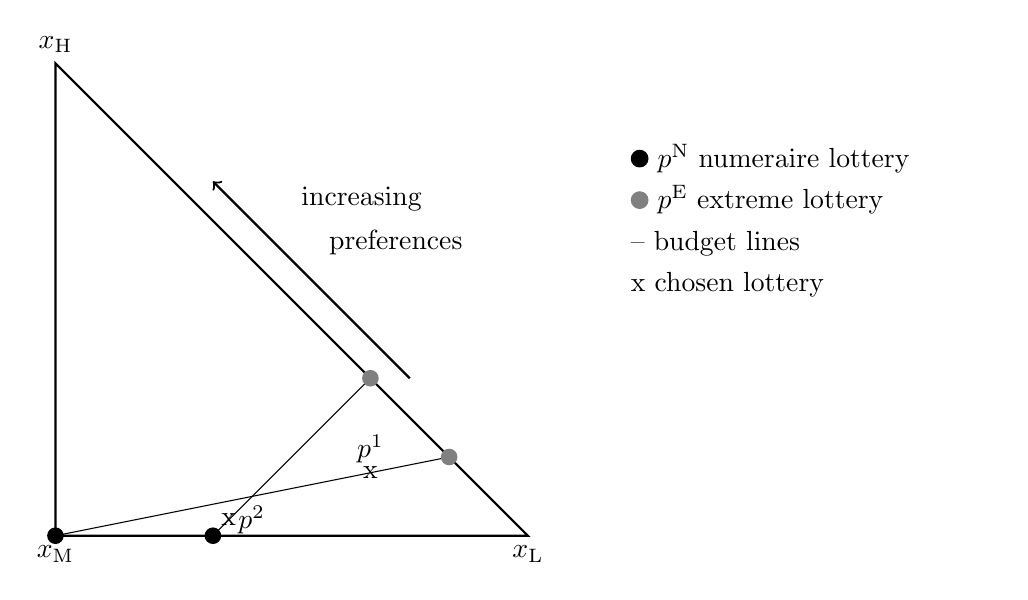
\begin{tikzpicture}
	%M-M triangle
	\draw[thick] (0,0) node[align=left,   below] {$x_{\midd}$}
		-- (0, 6) node[align=left,   above] {$x_{\hi}$}
		-- (6, 0) node[align=left,   below] {$x_{\low}$}
		--cycle;

	%Improving Preferences
	\draw[->,thick] (4.5,2) -- (2,4.5);
	\draw (3,4) node[align=left,   right] {increasing\\[.1em] \quad preferences};

	%Draw three budgets
	%% Lines
	\draw (0,0)--(5,1);
	\draw (2,0)--(4,2);

	%% p^{\edw}
 	\fill[black] (0,0)  circle[radius=3pt];
	\fill[black] (2,0)  circle[radius=3pt];
	
	%% Second p^{srd}
	\fill[gray] (4,2)  circle[radius=3pt];
	\fill[gray] (5,1)  circle[radius=3pt];

	%Mark the chosen bundles
	\draw (4,.8) node {x};
	\draw (4,.8)  node[align=left, above] {$p^1$};
	\draw (2.2,.2) node {x};
	\draw (2.2,.2)  node[align=left, right] {$p^2$};

	%Legend
	\draw[xshift=12cm, yshift=4cm] node [ left,text width=13em]
   	 {
	\tikz\draw[black,fill=black] (0,0) circle (3pt); $p^{\edw}$ numeraire lottery \\
	\tikz\draw[gray,fill=gray] (0,0) circle (3pt); $p^{\srd}$ extreme lottery\\
	-- budget lines \\
	x chosen lottery
  	  };
	\end{tikzpicture}
        \caption{Example of Choices that Cannot be Described by Preferences}
         \label{fig:warp}
\end{figure}

The revealed preference conditions prevent cycles of choices in the dataset that lead to an observation being strictly revealed preferred to itself. One example of data that is ruled out using the revealed preference conditions for a preference that satisfies FOSD is given in Figure~\ref{fig:warp}. Notice that if a lottery lies to the southeast of the budget set, then (assuming first order stochastic dominance) it is less preferred to the chosen mixture.\footnote{This follows since any points to the north or west of a point to the southeast of the budget line are strictly preferred by first order stochastic dominance. Making enough movements north or west will eventually lead to a point on the budget line. Finally, the point on the budget line is weakly less preferred to the chosen point by transitivity.} Thus, the choices from Figure~\ref{fig:warp} generate a strict cycle where lottery $p^1$ is strictly preferred to $p^2$ and lottery $p^2$ is strictly preferred to $p^1$, which is impossible for a well-defined preference relation.

Using the revealed preference approach, we find 14/144 (9.7\%) subjects have behavior that is described by a well-defined preference relation that satisfies FOSD. We find that most behavior cannot be exactly described by a preference relation. To account for this issue, we use the Houtman-Maks index (HMI) developed in \cite{houtman/1985} to find the largest number of choices that can be described by a preference relation. Here, a higher HMI indicates that behavior is closer to a well-defined preference relation conditional on the budget sets being the same. To better understand the HMI, note that the data in Figure~\ref{fig:warp} has an HMI of one since either observation can be removed, and the resulting dataset can be described by a preference relation.

We display a relative probability distribution of the HMI for all subjects in Figure~\ref{fig:HMIcomp} relative to some benchmark behavior following ideas from \cite{bronars/1987}. Recall, we model behavior for benchmark demand effects as simulated individuals choosing $\alpha$ according to the uniform distribution on $[45,55]$. Similarly, we model benchmark noisy behavior as simulated individuals choosing $\alpha$ according to the uniform distribution on $[0,100]$. For each case, we generate 5,000 simulated individuals. We plot the distribution of simulated HMI along with the distribution of subject HMI in Figure~\ref{fig:HMIcomp} for each benchmark.

\begin{figure}[H]
  \centering
      \begin{subfigure}[b]{0.48\textwidth}
        \includegraphics[width=\textwidth]{figs/HMIHistEDB.png}
        \caption{Demand Effect Benchmark}
    \end{subfigure}
    \begin{subfigure}[b]{0.48\textwidth}
        \includegraphics[width=\textwidth]{figs/HMIHistNB.png}
        \caption{Noisy Benchmark}
    \end{subfigure}
        \caption{HMI Probability Density of Subjects and Benchmark Behavior}\label{fig:HMIcomp}
    \raggedright
\end{figure}

First, we compare subject behavior to benchmark demand effects in Figure~\ref{fig:HMIcomp}(a). We see that subjects have many more choices that are  consistent with a preference relation that respects FOSD. In particular, we find that 144/144 (100\%) subjects are ``closer" to a well-defined preference than 95\% of simulated benchmark demand effect behavior according to the HMI. Moreover, we reject the null that the distribution of subject HMI and benchmark demand effects are the same according to the Wilcoxon rank sum test ($p<0.0001$) and according to the Kolmogorov-Smirnov test ($p<0.0001)$. We take this as evidence that demand effects are not substantive.

Next, we compare subject behavior to benchmark noise in Figure~\ref{fig:HMIcomp}(b). For this case, we find that 141/144 (97.9\%) subjects are ``closer" to a well-defined preference than 95\% of simulated benchmark noisy behavior according to the HMI. Moreover, we reject the null that the distribution of subject HMI and benchmark noisy behavior are the same according to the Wilcoxon rank sum test ($p<0.0001$) and according to the Kolmogorov-Smirnov test ($p<0.0001)$. We take this as evidence that the individuals are revealing information about their preferences.\footnote{In the spirit of \cite{andreoni/etal/2017} we also compare subject behavior to bootstrapped samples and find similar qualitative results. See Appendix~\ref{apn:benchmark} for details.} Thus, this interface may be useful for eliciting behavior in other settings.

\section{Additional Results}\label{sec:addRes}
Now that we have presented the main results, we explore two other themes: aggregate demand for numeraire lotteries and individual preference heterogeneity. The first section shows that when there is a numeraire lottery whose price varies, aggregate behavior can be well fit by a linear-log demand function. In particular, a regression of demand $(\alpha)$ on log relative prices $(\log(r))$  provides a good fit of aggregate behavior. The second section briefly describes some ``types" of individual behavior that are present in the data. In particular, we find rich heterogeneity of individual behavior even in this small choice domain with three monetary prizes. 

\subsection{Demand Analysis}\label{sec:aggDemand}

As expressed in \citet{machina/1982,machina/1985}, the behavioral implications of non-expected utility theory share many similarities with standard consumer theory. We examine this claim for aggregate demand of the numeraire lottery against the relative price. Recall that the demand for the numeraire lottery can be represented by the amount of $\alpha$ chosen on the slide rule in the choice interface. In Figure~\ref{fig:demand}, we find that the average demand for the numeraire lottery approximately follows a downward sloping linear-log function when analyzing choices for reference lottery N2 (\$10 for certain).\footnote{This differs from the numeraire lottery being chosen less often in the presence of ``income effects" since here a numeraire lottery is fixed.} This result is robust for N1-N7 as shown in Appendix~\ref{apn:Aggdemand} with regression results and additional figures. Thus, we conclude that aggregate behavior of risk can be described by relatively simple demand systems that satisfy the familiar property of downward sloping demand.

\begin{figure}[H]
\centering
        \includegraphics[scale=.48]{figs/AggDemN2.png}
       \caption{Demand Behavior for Numeraire Against Relative Prices for N2}\label{fig:demand}
\end{figure}

\subsection{Behavior Patterns and Individual Heterogeneity}\label{sec:hetero}
While aggregate behavior is described by simple demand systems, there is heterogeneity in individual preferences. In Figure~\ref{fig:type}, we show the choices of six different individuals that represent different behavior in the convex choice tasks from numeraire lotteries N1, N2, and N5. The behavior of all individuals for all budgets in this graphical form is presented in Appendix~\ref{apn:AllBehavior}. The types of behavior we show in Figure~\ref{fig:type} are representative of most behavior in the data. While we believe performing a formal preference classification exercise is interesting, it would shift the focus of the paper. For example, one could use methods that have been previously used in the work of \cite{fudenberg2019predicting} and \cite{naecker/2017}.    

We briefly describe the different types of behavior from Figure~\ref{fig:type}. First, Figure~\ref{fig:type}(a) represents the only individual who can be represented by the expected utility model. As expected, all choices lie on the extreme points of the MM triangle. The behavior in Figure~\ref{fig:type}(b) and (c) can be seen as thresholding behavior around an iso-$p_{\midd}$ curve and local thresholding around iso-$p_{\low}$ curves respectively. We call this thresholding behavior because behavior is ``as if" an individual chooses some threshold amount of $p_{\midd}$ or $p_{\low}$ and chooses the mixture that gives the threshold amount.  Figure~\ref{fig:type}(d) represents a combination of multiple types of behavior.  Figure~\ref{fig:type}(e) is labeled price responsive since the choices gradually respond to prices. Finally, Figure~\ref{fig:type}(f) has no discernible pattern. 

Combining the large amount of individual preference heterogeneity with the downward sloping aggregate demand, we find support for the hypothesis of \cite{becker/1962} that aggregate demand is downward sloping even in the presence of preference heterogeneity in the domain of risk. 

\begin{figure}[!h]
  \centering
   \begin{subfigure}[b]{0.31\textwidth}
        \includegraphics[width=\textwidth]{figs/choice.triangles.E125/ind_choice2_E125_123.pdf}
        \caption{Expected Utility}
    \end{subfigure}
          \begin{subfigure}[b]{0.31\textwidth}
        \includegraphics[width=\textwidth]{figs/choice.triangles.E125/ind_choice2_E125_20.pdf}
        \caption{Middle Thresholding}
    \end{subfigure}
    \begin{subfigure}[b]{0.31\textwidth}
        \includegraphics[width=\textwidth]{figs/choice.triangles.E125/ind_choice2_E125_132.pdf}
	\caption{Low Thresholding}
    \end{subfigure}
    \begin{subfigure}[b]{0.31\textwidth}
        \includegraphics[width=\textwidth]{figs/choice.triangles.E125/ind_choice2_E125_143.pdf}
        \caption{Combination}\label{fig:type.combo}
    \end{subfigure}
    \begin{subfigure}[b]{0.31\textwidth}
        \includegraphics[width=\textwidth]{figs/choice.triangles.E125/ind_choice2_E125_11.pdf}
	\caption{Price Responsive}
    \end{subfigure}
    \begin{subfigure}[b]{0.31\textwidth}
        \includegraphics[width=\textwidth]{figs/choice.triangles.E125/ind_choice2_E125_62.pdf}
	\caption{Random}
    \end{subfigure}
       \caption{Example Individual Choice Behavior from Convex Tasks N1, N2, and N5}
       \label{fig:type}
\raggedright
\end{figure}

%%%%%%%%%%%%%%%%%%%%%%%%%%%%%%
\section{Related Literature}\label{sec:lit}
%%%%%%%%%%%%%%%%%%%%%%%%%%%%%%

This section discusses the relation of this paper to the literature on stochastic choice, risk preferences, and revealed preference. First, there are several papers that have examined stochastic choice from an experimental perspective. The work of \cite{mosteller/1951} was the first to find that individuals randomize when facing repeated discrete choice problems. \cite{sopher/narramore/2000} examine whether individuals choose mixtures of lotteries using a similar interface to this paper. Moreover, \cite{sopher/narramore/2000} examined repeated convex choice tasks with the same budget and found similar choices in the repetitions. They took this as evidence in support of a preference for randomization. We complement these papers by comparing the convex choice tasks to the repeated discrete choice tasks. We also have many more convex choice tasks and check revealed preference conditions to show that the interface from \cite{sopher/narramore/2000} is eliciting preference information.  

Modern work on stochastic choice experiments includes \cite{burghart/2019}, \cite{Agranov/Ortoleva/2017}, \cite{dwenger/etal/2018}, \cite{agranov2020stable}, and \cite{agranov2020ranges}. The work of \cite{burghart/2019} focuses on examining choices from convex discrete budgets and examines violations of the independence condition. The work of \cite{Agranov/Ortoleva/2017} and \cite{dwenger/etal/2018} both find a preference for purchasing external randomization devices. This evidence supports the idea that individuals have a preference for randomization. In particular, \cite{Agranov/Ortoleva/2017} find that a preference for the randomization device positively correlates with mixing behavior in repeated binary-choice tasks. \cite{agranov2020stable} show a positive correlation between mixing in strategic and non-strategic environments.\footnote{This paper also examines mixing between lotteries when first order stochastic dominance can be violated and finds correlation across strategic and non-strategic choices. We do not allow subjects to choose first order stochastic dominated lotteries.}  Finally, \cite{agranov2020ranges} show that individuals prefer to randomize for a range of monetary values of various lotteries. In all these papers, as well as this paper, there is evidence that individuals prefer mixtures either in convex choice tasks or repeated discrete choice tasks. This paper is unique in that it links behavior across the two domains through a within-individual design. 

Models of a preference for randomization have also garnered theoretical interest. The interpretation of stochastic choice generated by non-expected utility preferences was popularized by \cite{machina/1985}. Some recent papers that examine conditions to characterize different models that come from a preference for randomization include \cite{fudenberg2015stochastic}, \cite{cerreia2019deliberately}, and \cite{allen2019revealed}.\footnote{This contrasts from other interpretations of stochastic choices from random utility models in \cite{mcfadden1974measurement}, \cite{mcfadden1990stochastic}, \cite{mcfadden2005revealed}, and \cite{gul2006random}.} The evidence here provides some support that a non-linear risk preference may drive a preference for randomization in repeated discrete choices tasks. Moreover, there are modern demand systems developed in \cite{fosgerau2019inverse} that may be able to match behavior of non-linear risk preferences when there are more than three prizes. 

This experiment is also related to risk preferences more generally, but we do not further explore this relationship in depth here. For example, we find evidence that mixing behavior is common in convex choice tasks which supports non-expected utility theory \citep{machina/1982} that allows mixing. More specifically, mixing behavior supports the hypothesis that there are regions of risk preferences that are quasi-concave. We also note that individual behavior suggests that risk preferences may only be locally well-behaved. For example, it appears that the ``low thresholding" individual in Figure~\ref{fig:type}(c) may have different thresholds that depend on the location of the budget set. This suggests additional study is needed to understand whether global risk preferences or local risk preferences are more appropriate for applications.  

The evidence we find in this paper against expected utility also illuminates why there might be differences in estimates of risk preferences using different elicitation methods. The common method to measure risk preferences following \cite{holt2002risk} uses choice lists with discrete choice. However, both \cite{friedman/2018} and \cite{andreoni/kuhn/2018} find that the different methods to elicit risk preferences yield different parameter estimates. Our research suggests part of the discrepancy may be that individuals prefer mixtures which may induce randomization. This agrees with research by \cite{chew2019multiple} that shows switching behavior in repeated discrete choice is correlated with multiple switching behavior in choice lists.

Moreover, since we find risk preferences may only be locally well behaved, these discrepancies may also be caused by using a global model of risk preferences. While there are methods that use convex budgets to elicit risk preferences following \cite{Gneezy/Potters} and \cite{choi/etal/2007}, these are currently less popular since the methods are slightly more complicated. The research in this paper suggests that this complication may be worthwhile due to non-linearities in risk preferences. A promising approach that is close to existing practice is to use convex budgets with the choice list elicitation of \cite{Holt/Laury/2002}. Choices from these convex budgets also correlate with discrete choice behavior and are used in \cite{cettolin2019revealed} and \cite{agranov2020ranges}. 

Finally, this paper is related to experiments that take a revealed preference approach. General methods and theory of revealed preference are given a textbook treatment in \cite{chambers2016revealed}. There are now numerous papers that use revealed preference methods, including some mentioned earlier. Other experimental papers that take a revealed preference approach include, \cite{kagel1995economic} who examine the rationality of animals, \cite{andreoni2002giving} who examine altruistic behavior, \cite{andreoni2003bargainers} who examine bargaining behavior, \cite{choi/etal/2007} who examine Arrow securities, and \cite{andreoni2012estimating} who examine time preferences using convex budgets. Relative to this literature, our experimental methods are closest to \cite{andreoni2002giving}, \cite{andreoni2003bargainers}, and \cite{andreoni2012estimating} since we use a fixed set of budgets for all subjects. 

%%%%%%%%%%%%%%%%%%%%%%%%%%%%%%%%%%%%%%%%%%%%%%%%%%%%%%%%%%%%%%%

\section{Concluding Remarks}\label{sec:conclusion}

%%%%%%%%%%%%%%%%%%%%%%%%%%%%%%%%%%%%%%%%%%%%%%%%%%%%%%%%%%%%%%%

We designed an experiment to examine the prevalence of mixing behavior and examine whether behavior from convex choice tasks is related to behavior from repeated discrete choice tasks. Our exploratory study shows that mixing behavior is common and that behavior from repeated discrete choice tasks mimics behavior from convex choice tasks. We also show that the interface provided in this paper can elicit information on non-linear risk preferences. While these results are suggestive that risk preferences may drive a preference for randomization in repeated discrete choice tasks, we believe more work is needed to see the extent of this relation. For example, interesting follow-up research could examine additional comparisons between convex budgets and repeated discrete choice tasks at different prices or examine how increasing the number of repetitions affects the closeness to the convex choice task. We also hope this motivates additional theoretical research following the work of \cite{lu2019repeated} that looks at how repeated discrete choices are related to risk preferences.

%%%%%%%%%%%%%%%%%%%%%%%%%%%%%%%%%%%%%%%%%%%%%%%%%%%%%%%%%%%%%%%


\newpage 

\bibliography{Bibliography2}
\bibliographystyle{aer}

\newpage
[Supplemental Material]

\begin{appendices}

\section{Experimental Instructions}\label{app:inst}

Each instruction page was read out loud and subjects were instructed not to click ahead. The full set of instructions appears below. After the first set of instructions, there was a short series of training examples. Static versions of the training tasks appear in Figures \ref{ex1} - \ref{ex4}. After the training tasks, payments were explained using each subject's final training exercise. An example is depicted in Figure~\ref{earn}. Important points were emphasized as ``Things to Remember." Part I is for the convex choice tasks and part II is for the repeated discrete choice tasks. After all tasks from part I were completed, a second set of instructions was given for part II. Once the task that pays was determined, a subject could examine it to observe their choices from the task. An example of this page appears in Figure~\ref{dtc}.

\textbf{[Instructions:]}
\small{
 \textbf{ PLEASE READ CAREFULLY AND DO NOT PRESS NEXT UNTIL INSTRUCTED TO DO SO.}
 
    This is a study about your own preferences. There are no right or wrong answers. This study has two parts.
    Part I has 79 tasks and Part II has 6 tasks. Once you have finished,
    we will pick a Task at random as the  \textbf{Decision-that-counts}. Since all decisions are equally
    likely to be chosen, you should approach each task as if it is the  \textbf{Decision-that-counts}. Part II will be
    explained once you complete Part I.
 
    For Part I your objective in each of the 79 tasks is to pick the  \textbf{Chance} that you like the most. Every task
    has a changing visual aid to assist with picking your preferred  \textbf{Chance}.
 

 
    In every task, you must choose among the different  \textbf{Chances} of receiving three prizes.
    The three prizes are \$2, \$10 and \$30. Each  \textbf{Chance} will assign different chances to the three prizes.
    To determine your preferred chance, and all possibilities, you will have to move a slider. For all tasks,
    picking 100 will always give you the largest chance of the middle prize of \$10. As you move the slider towards 0,
    the chance of both \$30 and \$2 will increase. The largest chance of \$10 and how the other two chances change,
    as you move the slider, will be different for different tasks.
 

 
    Most  \textbf{Chances} might involve some risk. For example, a  \textbf{Chance} could be a 25 in 100 chance of \$30,
    a 50 in 100 chance of \$10, and a 25 in 100 chance of \$2 while  another  \textbf{Chance} could be a 100 in 100 chance,
    or a sure prize, of \$10. To aid with your choice, there will be a changing display for every possible  \textbf{Chance}.
    Therefore, for any  \textbf{Chance} you will always be able to see the chance of receiving each
    of the prizes.
 

 
    The next few pages contains 4 examples to familiarize you with ``How this works". The examples have prizes that are
    different from the main tasks. Take your time and make sure you understand ``How it works". We will not begin until
    everybody completes these examples and payments are explained. After the examples, there will be a detailed
    explanation of how payments will be determined.
 
 
     \textbf{Important}: You must move the slider around and then verify your answer next to it.
    If the chosen  \textbf{Chance} on the slider does not match the  \textbf{Verified Chance} next to it,
    or if you do not move the slider around, you will not be allowed to proceed to the next task.
    Once you have picked a  \textbf{Chance} for a given task and verified it, you will no longer
    be able to change it.
 

 
     \textbf{Very Important:} For each task, the slider is a tool to help you decide the choice you like the best.
    Therefore, it is in your best interest to move it around to help you determine which  \textbf{Chance} you like better.
 }

\textbf{[Examples 1-4]}

\begin{figure}[H]
  \centering
  	\begin{subfigure}[b]{0.45\textwidth}
  	\includegraphics[width=.7\textwidth,angle=-90]{figs/ex1_g.pdf}
        \caption{Example 1}\label{ex1}
	\end{subfigure}
	 \begin{subfigure}[b]{0.45\textwidth}
  	\includegraphics[width=.7\textwidth,angle=-90]{figs/ex2_g.pdf}
        \caption{Example 2 }
	\end{subfigure}
	%\caption*{Examples 1 and 2}\label{ex12}
\end{figure}

\begin{figure}[H]
  \centering
  	\begin{subfigure}[b]{0.45\textwidth}
  	\includegraphics[width=.7\textwidth,angle=-90]{figs/ex3_g.pdf}
        \caption{Example 3} \label{ex3}
	\end{subfigure}
	 \begin{subfigure}[b]{0.45\textwidth}
  	\includegraphics[width=.7\textwidth,angle=-90]{figs/ex4_g.pdf}
        \caption{Example 4 } \label{ex4}
	\end{subfigure}
	%\caption*{Examples 3 and 4}\label{ex34}
\end{figure}

\newpage 

\textbf{[Earning Money:]}
\begin{figure}[H]
  \centering
  	\includegraphics[width=.7\textwidth]{figs/earn_g.png}
        \caption{How to Earn Money}
        \label{earn}
\end{figure}

\pagebreak

\textbf{[Things to Remember:]}

 \small{
 \textbf{PLEASE READ CAREFULLY AND DO NOT PRESS NEXT UNTIL INSTRUCTED TO DO SO.}
 
\begin{itemize}
 
\item You will complete 79 tasks for Part I. Part II has 6 tasks and will be explained after Part I.
 

 
\item Different  \textbf{Chances} will determine a different chance for each prize. All you have to
    do is pick the  \textbf{Chance} you like the best.
 
 
\item There is no right or wrong answer for any of these questions. We are interested in studying your preferences.
 

 
\item Once all of your decisions have been made, we will choose one task and one
decision as the decision-that-counts and will implement your preferred  \textbf{Chance}.
 

 
\item Every decision is equally likely to be the  \textbf{Decision-that-counts}. So, it is in your
interest to treat each  \textbf{Chance} as if it could be the one that determines your
payoffs.
 
 
\item For each task, you must move the slider and verify your preferred  \textbf{Chance}. Failure
    to move the slider or not match it will prevent you from moving to the next task.
 
 
\item Once you have selected your preferred  \textbf{Chance} and verified it, you will not be able to
    change it.
 
 
\item The slider is a tool to help you determine your preferred  \textbf{Chance}.
    Therefore, it is in your best interest to use it to evaluate all potential alternatives.
 
\end{itemize}
}

\textbf{[Part I: Tasks 1-79] Occurs here}

\small{
 \textbf{PLEASE READ CAREFULLY AND DO NOT PRESS NEXT UNTIL INSTRUCTED TO DO SO.}
 
    In this part of the study you are asked again to choose your preferred  \textbf{Chance}, just like you did in Part I. The
    difference between this Part and Part I is that in this part you will see the same question three times, one after
    the other. That is: you will be asked one question; once you click the Next button, you will be asked the
    same question again; and once you click the Next button, the same question will appear for the third time. Once
    you click the Next button, then a new question will appear, which will also be asked three times. There are a total
    of 2 questions, each asked three times, for a total of 6 tasks.
 

 
    Another difference is that you will only be able to choose between two  \textbf{Chances}, 0 or 100. Please remember
    that there is no right or wrong answer. Remember you must move the slider around and then verify your answer next to it.
    If the chosen  \textbf{Chance} on the slider does not match the  \textbf{Verified Chance}, or if you do not move
    the slider around, you will not be allowed to proceed to the next task. Once you have picked a  \textbf{Chance} for a
    given task and verified it, you will no longer be able to change it.
}

\textbf{[Part II: Tasks 80-85] Occurs here}

\begin{figure}[H]
  \centering
  	\includegraphics[width=.5\textwidth, angle=-90]{figs/dtc_g.pdf}
        \caption{Decision-that-counts}\label{dtc}
\end{figure}

\section{Pay one decision incentives}\label{app:payone}

We pay one decision following the intuition of \cite{azrieli/etal/2018, healy/2019} who build on the work of \cite{Karni/Safra/1987} and \cite{segal1990two}. We discuss how our payment scheme maps into these papers after describing how payment uncertainty is resolved. Uncertainty is resolved using physical randomization devices. Each task could be chosen for payment with equal probability. We reminded subjects of this during each task. Before starting the discrete choice tasks, subjects were informed they would face the same binary choice three times in a row. They were also told there were two different binary choices for a total of six tasks. After the decisions from the convex and discrete choice tasks were completed, a ten-sided dice was rolled twice, once for the tens digit and another for the ones digit, to determine the task that counts. Any number above 85 was re-rolled. Subjects entered the chosen task into the computer terminal and were reminded about their choice for that task and the resulting distribution over payoffs from that choice. 

To determine payoffs for the chosen task, four ten-sided dice were rolled. So a roll of 5, 6, 7, and 9 would give 56.79\%. The chosen distribution induced at most three intervals $[0,x)$, $[x,y)$, and $[y,1]$ for the low, middle, and high prize respectively. When a binary task was chosen for payment or the convex choice was at a corner, only two intervals applied to the relevant prizes. The interval that contained the number determined which outcome was obtained. To induce greater variation in outcomes, four sets of four dice were rolled. Each set of four dice applied to at most six subjects.

Finally, we relate the resolution of lotteries from the experiment to the pay one scheme discussion in \cite{azrieli/etal/2018}. Here, we assume the die roll to select a task that pays induces a compound lottery over the objective lotteries used in the experiment. Thus, the result of the die roll can be viewed as a state using the notation of \cite{azrieli/etal/2018}. We assume that the individual satisfies first order stochastic dominance over the prizes in this state space. Finally, we assume that the individual is able to internally randomize according to their most preferred distribution following the interpretation of \cite{machina/1985}. Thus, we assume each ``choice" in the repeated discrete choice tasks is an independent draw from an individual's most preferred distribution. This last assumption is implicit in \cite{Agranov/Ortoleva/2017}.

\section{Revealed Preference Results}\label{apn:rp}

Here we provide a revealed preference characterization for a utility model of risk preferences that respects first order stochastic dominance for lotteries with three monetary prizes. The results are similar to those of \cite{varian/1982}, \cite{forges2009afriat}, \cite{heufer/2013}, and \cite{cerreia/etal/2018}. We consider risk preferences over lotteries with three monetary prizes that are ordered $x_{\low} < x_{\midd}< x_{\hi}$. The probability that the prizes $x_{\low}, x_{\midd},$ and $x_{\hi}$ occur are denoted $p_{\low}, p_{\midd},$ and $p_{\hi}$ respectively. Moreover, let $\Delta=\{ p \in \mathbb{R}_+^3 \mid p_{\low}+p_{\midd}+p_{\hi}=1\}$ be the probability simplex for three prize lotteries.  

We consider budget sets generated by convex combinations of a numeraire lottery $p^{\edw}$ and extreme lotttery $p^{\srd}$. Here the budgets are given by
\begin{align*}
B(p^{\edw},p^{\srd}) = 
\left\{ 
  \begin{aligned}
 p=(p_{\low}, p_{\midd}, p_{\hi}) \in \mathbb{R}_{+}^3 &\mid  p_{\hi} - r(p^{\edw},p^{\srd}) p_{\low} \le p_{\hi}^{\edw} - r(p^{\edw},p^{\srd}) p_{\low}^{\edw}  \\
&\mid\quad p_{\low} + p_{\midd} + p_{\hi} =1  
  \end{aligned}
\right\}
 \end{align*}
where $r(p^{\edw},p^{\srd})=\frac{p_{\hi}^{\srd}-p_{\hi}^{\edw}}{p_{\low}^{\srd}-p_{\low}^{\edw}}$ is the relative price of the numeraire lottery described in the main text. Recall, we consider  $r(p^{\edw},p^{\srd})\in \mathbb{R}_{++}$ since we are only considering budget sets that do not have lotteries ordered by FOSD. 

Let $\{ p^t , B( p^{\edw,t}, p^{\srd,t}) \}_{t=1}^{T}$ be a dataset generated by an individual choosing the lottery $p^t$ from the budget $B( p^{\edw,t}, p^{\srd,t})$ where $ p^{\edw,t}$ is the numeraire lottery from the $t$-th task and $p^{\srd,t}$ is the extreme lottery from the $t$-th task. We will often abbreviate the price so that $r^t=r(p^{\edw,t},p^{\srd,t})$. Our main focus is to find conditions that determine when the choices an individual makes can be described by a utility function that satisfies first-order stochastic dominance. Recall, the lottery $p'=(p_{\low}',p_{\midd}', p_{\hi}')$ first order stochastic dominates the lottery $p=(p_{\low},p_{\midd}, p_{\hi})$ when $p'_{\hi}\ge p_{\hi}$ and $p'_{\hi}+p'_{\midd} \ge p_{\hi}+p_{\midd}$ with at least one inequality strict.

\begin{definition}
The dataset $\{ p^t , B( p^{\edw,t}, p^{\srd,t}) \}_{t=1}^{T}$ is first-order stochastic dominance rationalized by a utility function when there exists a utility function $V : \Delta \rightarrow \mathbb{R}$ such that
\begin{enumerate}
\item For all $t \in \{1,\ldots, T\}$,
	\[ p^t \in \argmax_{ p \in B( p^{\edw,t}, p^{\srd,t}) } V(p) ;\]
\item For all $p'$ that first-order stochastic dominate $p$, 
	\[ V(p') > V(p) .\]
\end{enumerate}
\end{definition}

Now we define revealed preference relations for the lotteries above. We say that a lottery $p^t$ is \emph{directly revealed preferred} to the lottery $p^s$, denoted $p^t \mathbin{R} p^s$, if $p_{\hi}^s-r^t p_{\low}^s\le p_{\hi}^{\edw,t}-r^t p_{\low}^{\edw,t}$. We are able to use the terms for the numeraire lottery to define a revealed preference relation when looking for a first-order stochastic dominance utility rationalization since the lottery chosen from budget $t$ must satisfy 
\[ p_{\hi}^t - r^t p_{\low}^t = p_{\hi}^{\edw,t} - r^t p_{\low}^{\edw,t} .\] 

To see this, suppose by contradiction that 
\[ p_{\hi}^t - r^t p_{\low}^t < p_{\hi}^{\edw,t} - r^t p_{\low}^{\edw,t} .\]
In this case, one can find a lottery $p'$ that first order stochastic dominates $p^t$ and is still feasible in $B( p^{\edw,t}, p^{\srd,t})$. For example, let $p_{\hi}' > p_{\hi}^{t}$, $p_{\hi}' + p_{\mid}' = p_{\hi}^{t}+p_{\mid}^t$, and 
\[ p_{\hi}' - r^t p_{\low}' = p_{\hi}^{\edw,t} - r^t p_{\low}^{\edw,t} .\]
This lottery first order stochastic dominates $p^t$ which contradicts the data coming from a utility function that satisfies first-order stochastic dominance.  
Next, we say a lottery $p^t$ is \emph{directly strictly revealed preferred} to the lottery $p^s$, denoted $p^t \mathbin{P} p^s$, if $p_{\hi}^s-r^t p_{\low}^s < p_{\hi}^{\edw,t}-r^t p_{\low}^{\edw,t}$. We say that lottery $p^t$ is \emph{revealed preferred} to the lottery $p^s$, denoted $p^t \mathbin{R}^{*} p^s$, is there exists a sequence $\{ m \}_{m=1}^M$ with $M\ge 2$ such that $p^{1}=p^t$ and $p^{M}=p^s$ such that $p^m \mathbin{R} p^{m+1}$ for all $m=1,\ldots,M-1$. Similarly, we say that the lottery $p^t$ is \emph{strictly revealed preferred} to the lottery $p^s$, denoted $p^t \mathbin{P}^{*} p^s$, is there exists a sequence $\{ m \}_{m=1}^M$ with $M\ge 2$ such that $p^{1}=p^t$ and $p^{M}=p^s$ such that $p^m \mathbin{R} p^{m+1}$ for all $m=1,\ldots,M-1$ where for some $m\in\{1,\ldots,M-1\}$ there is a strict preference revelation so that  $p^m \mathbin{P} p^{m+1}$.

The revealed preference relation generated from the dataset is \emph{acyclic} when 
\[ p^t \mathbin{R}^{*} p^{s} \; \text{implies} \quad \text{not}\; p^s \mathbin{P} p^t.\] 
We mention that $\text{not}\; p^s \mathbin{P} p^t$ is the same as $p_H^t-r^s p_L^t \ge p_H^s - r^s p_L^s$. Acyclicity of a revealed preference relation is similar to  the generalized axiom of revealed preference from \cite{varian/1983}. In particular, acyclicity requires that a researcher cannot find a cycle of lotteries such that a lottery is strictly revealed preferred to itself. We say there is a cycle when there exists a sequence $\{t_m\}_{m=1}^M$ with $M\ge 2$ where $t_m \in \{1,\ldots, T\}$ such that $p^{t_m} \mathbin{R} p^{t_{m+1}}$ for all $m=1,\ldots,M-1$ and $p^{t_M} \mathbin{P} p^{t_1}$.

\begin{proposition}
The following are equivalent for the dataset $\{ p^t , B( p^{\edw,t}, p^{\srd,t}) \}_{t=1}^{T}$ when all $r^t >0$:
\begin{enumerate}
	\item The dataset is first-order stochastic dominance  rationalized;
	\item The revealed preference relations generated from $\mathbin{R}$ and $\mathbin{P}$ satisfy acyclicity;
	\item For all $t \in \{1,\ldots,T\}$ there exist numbers $u^t \in \mathbb{R}$ and $\lambda^t \in \mathbb{R}_{++}$ such that for all $s,t \in \{1,\ldots, T \}$
	\[ u^s \le u^t + \lambda^t\left( p_{\hi}^s - p_{\hi}^{\edw,t} - r^t( p_{\low}^s - p_{\low}^{\edw,t} ) \right) ;\]
	\item The dataset is first-order stochastic dominance rationalized with a continuous and concave utility function. 
\end{enumerate}
\end{proposition}

\begin{proof}
$(1)\implies (2)$ Suppose by contradiction that the dataset is FOSD rationalized and the revealed preference relation has a cycle for observations $\{t_m\}_{m=1}^M$ where $t_m \in \{1,\ldots,T\}$ so that 
\[\text{for}\; m=1\ldots,M-1 \quad  p^{t_m} \mathbin{R} p^{t_{m+1}} \quad \text{and}  \quad p^{t_M} \mathbin{P} p^{t_1}.\]
It follows that 
\[ V(p^{t_1}) \ge V(p^{t_2}) \ge \ldots \ge V(p^{t_M}) > V(p^{t_1}) \]
where the strict inequality holds since $p^{t_M} \mathbin{P} p^1$. However, this contradicts the existence of a well defined utility function.\\

$(2) \implies (3)$ This follows from the arguments in \cite{fostel2004two}, \cite{forges2009afriat}, or \cite{chambers2016revealed}.\\

$(3) \implies (4)$ We construct a utility function from the numbers $u^t$ and $\lambda^t$ that rationalize the data. In particular, consider the function 
\[ \tilde{V}(p) = \min_{t \in \{1,\ldots, T\} } \left\{ u^t + \lambda^t\left( p_{\hi} - p_{\hi}^{\edw,t} - r^t( p_{\low} - p_{\low}^{\edw,t} ) \right) \right\} .\]
It follows immediately that $\tilde{V} : \Delta^2 \rightarrow \mathbb{R}$ is continuous and concave since it is the minimum of finitely many affine functions. It remains to show the function satisfies first order stochastic dominance and satisfies the optimality properties. 

First, we show that the function satisfies first order stochastic dominance. To see this, note that if $p'$ first order stochastic dominates $p$, then $p_{\hi}' \ge p_{\hi}$ and $p_{\hi}' + p_{\midd}' \ge p_{\hi}+p_{\midd}$ with one inequality strict. Let $t' \in \{1,\ldots, T\}$ be chosen so \[ \tilde{V}(p')=u^{t'}+\lambda^{t'}\left( p_{\hi} - p_{\hi}^{\edw,t'} - r^{t'}( p_{\low} - p_{\low}^{\edw,t'} ) \right) .\]

We now show that first order stochastic dominance holds. It follows that
\begin{align*}
\tilde{V}(p')&=u^{t'}+\lambda^{t'}\left( p_{\hi}' - p_{\hi}^{\edw,t'} - r^{t'}( p_{\low}' - p_{\low}^{\edw,t'} ) \right) \\
        &> u^{t'}+\lambda^{t'}\left( p_{\hi} - p_{\hi}^{\edw,t'} - r^{t'}\left( p_{\low} - p_{\low}^{\edw,t'} \right) \right)\\
        &\ge \min_{t \in \{1,\ldots, T\} }\left\{ u^t + \lambda^t\left( p_{\hi} - p_{\hi}^{\edw,t} - r^t\left( p_{\low} - p_{\low}^{\edw,t} \right) \right) \right\} \\
        &= \tilde{V}(p)
\end{align*}
where the strict inequality follows since either $p_{\hi}' > p_{\hi}$ or $p_{\hi}' + p_{\midd}' > p_{\hi}+p_{\midd}$. When $p_{\hi}' > p_{\hi}$, the the strict inequality holds since $\lambda^{t'}>0$, $r^t>0$, and $0 \le p_{\low}' \le p_{\low}$ . When $p_{\hi}' + p_{\midd}' > p_{\hi}+p_{\midd}$, this implies that $p_{\low}'<p_{\low}$ and the the strict inequality holds since $\lambda^{t'}>0$, $r^t>0$, and $0 \le p_{\hi} \le p_{\hi}'$.

Finally, we show that the lotteries $p^s$ are optimal for the given budgets. Note that for any lottery $p \in B( p^{\edw,s}, p^{\srd,s})$ that 
\begin{align*}
    \tilde{V}(p) &= \min_{t \in \{1,\ldots, T\} } \left\{ u^t + \lambda^t\left( p_{\hi} - p_{\hi}^{\edw,t} - r^t( p_{\low} - p_{\low}^{\edw,t} ) \right) \right\} \\
        &\le u^s + \lambda^s\left( p_{\hi} - p_{\hi}^{\edw,s} - r^s( p_{\low} - p_{\low}^{\edw,s} ) \right)\\
        &\le u^s\\
        &= \tilde{V}(p^s)
\end{align*}
where the second inequality follows since $p_{\hi} - r^s p_{\low} \le p_{\hi}^{\edw,s} - r^s p_{\low}^{\edw,s}$ and $\tilde{V}(p^s)=u^s$ by the construction of the inequalities in (2).\\

$(4)\implies(1)$ is immediate. 
\end{proof}

This proof follows from standard arguments in revealed preference. This is also related to work by \cite{nishimura2017comprehensive} who give conditions for when there is a preference relation that preserves a partial order such as first order stochastic dominance. Relative to the more general revealed preference analysis from \cite{nishimura2017comprehensive}, \cite{heufer/2013}, and \cite{cerreia/etal/2018} we are able to get a continuous and concave utility representation because we focus on finite dimensional lotteries and the budget sets we use here are convex.

In order to measure violations of a first-order stochastic dominance rationalization, we use the Houtman-Maks index (HMI). The HMI is proposed in \cite{houtman/1985} and suggests using the largest number of choices that can be rationalized as a measure of closeness. Here, we find the largest number of choices that admit a first-order stochastic dominancee rationalization. We interpret a higher HMI to mean an individual is ``closer" to a first-order stochastic dominance rationalization since more data is consistent with this type of preference relation. While finding the HMI is a difficult problem in general, \cite{demuynck2021computing} shows that a mixed integer linear programming can quickly find the largest number of choices that can be rationalized for general budget sets. We present how to compute the HMI in the following proposition.

\begin{proposition}
The HMI for the dataset $\{ p^t , B( p^{\edw,t}, p^{\srd,t}) \}_{t=1}^{T}$ is computed by solving 
\begin{align*}
    \text{HMI} &=\max_{\substack{ A_t \in \{0,1\} \\
    U_{t,v} \in \{0,1\} \\ u_t \in [0,1] } } \; \sum_{t=1}^T A_t &\; \\
	\text{s.t.}\quad &\; u_t-u_v  \le -\varepsilon + 2U_{t,v} &\;  \forall t,v \in \{1,\ldots, T \}   \\
	&\;	U_{t,v}-1 \le u_t -u_v &\quad  \forall t,v \in \{1,\ldots, T \}  \\
	&\; -\left( p_{\hi}^v-r^t p_{\low}^v - p_{\hi}^{\edw,t} + r^t p_{\low}^{\edw,t} \right) \le -\delta + \beta(U_{t,v}+(1-A_t)) &\quad  \forall t,v \in \{1,\ldots, T \}  \\
	&\; \beta(U_{v,t}+A_t-2)\le \left( p_{\hi}^v-r^t p_{\low}^v - p_{\hi}^{\edw,t} + r^t p_{\low}^{\edw,t} \right) &\quad  \forall t,v \in \{1,\ldots, T \} 
\end{align*}
		where $0<\varepsilon < \frac{1}{T}$, $\beta > \max_{t,v\in \{1,\ldots,T\} } \left\{ \left|p_{\hi}^v-r^t p_{\low}^v - p_{\hi}^{\edw,t} + r^t p_{\low}^{\edw,t}\right| \right\} + \alpha$, and $0<\delta<\alpha$ where $\alpha =\min\{1, \min_{t,v}\{p_{\hi}^v - p_{\hi}^{\edw,t} - r^t( p_{\low}^v - p_{\low}^{\edw,t} ) \mid p_{\hi}^v - p_{\hi}^{\edw,t} - r^t( p_{\low}^v - p_{\low}^{\edw,t} ) > 0 \} \}$.
\end{proposition}

This proposition follows from \cite{demuynck2021computing}(Corollary 7). We compute the measure using the mixed integer linear solving from \cite{gurobi} through Matlab. The HMI for each individual is given in Table~\ref{tab:HMI_subs}.

\begin{table}[H]
\centering
\small
\begin{tabular}{cc}
 \toprule
(i)ndividual & HMI\\
\midrule
 1 & 70\\ 2 & 74\\ 3 & 76\\ 4 & 76\\ 5 & 78\\ 6 & 76\\ 7 & 75\\ 8 & 63\\ 9 & 75\\ 10 & 74\\ 11 & 79\\ 12 & 75\\ 13 & 77\\ 14 & 73\\ 15 & 68\\ 16 & 71\\ 17 & 71\\ 18 & 78\\ 19 & 63\\ 20 & 52\\ 21 & 74\\ 22 & 69\\ 23 & 72\\ 24 & 76\\ 25 & 71\\ 26 & 78\\ 27 & 71\\ 28 & 79\\ 29 & 77\\ 30 & 75\\ 
  \bottomrule
\end{tabular}
\begin{tabular}{cc}
 \toprule
i & HMI\\
 \midrule
 31 & 76\\ 32 & 79\\ 33 & 72\\ 34 & 73\\ 35 & 68\\ 36 & 66\\ 37 & 65\\ 38 & 77\\ 39 & 70\\ 40 & 75\\    41 & 76\\ 42 & 72\\ 43 & 63\\ 44 & 79\\ 45 & 74\\ 46 & 72\\ 47 & 77\\ 48 & 76\\ 49 & 71\\ 50 & 71\\ 51 & 65\\ 52 & 71\\ 53 & 79\\ 54 & 72\\ 55 & 75\\ 56 & 79\\ 57 & 66\\ 58 & 60\\ 59  & 72\\ 60 & 74 \\
 \bottomrule
\end{tabular}
\begin{tabular}{cc}
 \toprule
i & HMI\\
 \midrule
 61 & 71\\ 62 & 60\\ 63 & 79\\ 64 & 54\\ 65 & 76\\ 66 & 58\\ 67 & 74\\ 68 & 73\\ 69 & 78\\ 70 & 72\\ 71 & 60\\ 72 & 77\\ 73 & 73\\ 74 & 75\\ 75 & 76\\ 76 & 72\\ 77 & 65\\ 78 & 70\\ 79 & 74\\ 80 & 68\\ 81 & 70\\ 82 & 76\\ 83 & 71\\ 84 & 76\\ 85 & 78\\ 86 & 71\\ 87 & 75\\ 88 & 75\\ 89 & 75\\ 90 & 60\\ 
\bottomrule
\end{tabular}
\begin{tabular}{cc}
 \toprule
i & HMI\\
\midrule
91 & 62\\ 92 & 68\\ 93 & 79\\ 94 & 79\\ 95 & 75\\ 96 & 65\\ 97 & 74\\ 98 & 63\\ 99 & 75\\ 100 & 69\\ 101 & 61\\ 102 & 77\\ 103 & 77\\ 104 & 79\\ 105 & 79\\ 106 & 72\\ 107 & 74\\ 108 & 79\\ 109 & 69\\ 110 & 65\\ 111 & 78\\ 112 & 70\\ 113 & 68\\ 114 & 77\\ 115 & 72\\ 116 & 78\\ 117 & 67\\ 118 & 74\\ 119 & 64\\ 120 & 72\\ 
\bottomrule
\end{tabular}
\begin{tabular}{cc}
 \toprule
i & HMI\\
\midrule
121 & 74\\ 122 & 68\\ 123 & 79\\ 124 & 73\\ 125 & 78\\ 126 & 72\\ 127 & 77\\ 128 & 78\\ 129 & 69\\ 130 & 75\\ 131 & 70\\ 132 & 76\\ 133 & 78\\ 134 & 70\\ 135 & 72\\ 136 & 77\\ 137 & 76\\ 138 & 67\\ 139 & 71\\ 140 & 75\\ 141 & 78\\ 142 & 73\\ 143 & 68\\ 144 & 79\\ & \\ & \\
& \\ & \\ & \\ & \\ 
\bottomrule
\end{tabular}
\caption{Houtman-Maks Index for All Subjects}\label{tab:HMI_subs}
\end{table}

\subsection{Benchmark Behavior}\label{apn:benchmark}
Following the discussion in the main text, we compare the number of violations in the data from subjects to benchmarks of alternative behavior following the suggestion of \cite{bronars/1987}. In particular, we generate simulated choices $p^t$ from $B( p^{\edw,t}, p^{\srd,t})$ by choosing an $\alpha^t$ that generates choices following Equation~\ref{eq:alpha}. Following \cite{andreoni/etal/2017}, we also consider sampling over the distribution of choices in the population. Thus, let $\alpha^{i,t}$ be the choice of $\alpha$ by the $i$-th individual in the $t$-th task from the experiment. We generate simulated benchmarks the following four ways.
\begin{enumerate}
    \item Let $\alpha^t$ be distributed $U[45,55]$.
    \item Let $\alpha^t$ be distributed $U[0,100]$.
    \item Let $\alpha^t$ be distributed uniformly over $\{\alpha^{i,t}\}_{i,t}$.
    \item Let $\alpha^t$ be distributed uniformly over $\{\alpha^{i,t}\}_i$.
\end{enumerate}

The first randomization scheme is our benchmark demand effects setting where an individual ``trembles" around the initialized slide rule. The second  randomization scheme is an implementation of a \cite{bronars/1987} uniform random scheme and is our benchmark of noise. The third and fourth benchmarks follow \cite{andreoni/etal/2017} who suggest comparing behavior of individuals relative to randomness that is likely to be generated by individuals. We call the third randomization scheme a bootstrap benchmark since it bootstraps from all choices. Similarly, we call the fourth randomization scheme a conditional bootstrap benchmark since it bootstraps from choices conditional on a budget. We plot the distribution of simulated HMI along with the distribution of subject HMI for the third and fourth randomization schemes in Figure~\ref{fig:HMIcomp2}.

\begin{figure}[H]
  \centering
      \begin{subfigure}[b]{0.48\textwidth}
        \includegraphics[width=\textwidth]{figs/HMIHistA1.png}
        \caption{Bootstrap Benchmark}
    \end{subfigure}
    \begin{subfigure}[b]{0.48\textwidth}
        \includegraphics[width=\textwidth]{figs/HMIHistA2.png}
        \caption{Conditional Bootstrap Benchmark}
    \end{subfigure}
        \caption{HMI Probability Density of Subjects and Benchmark Behavior}\label{fig:HMIcomp2}
    \raggedright
\end{figure}

We compare subject behavior to the bootstrap benchmark in Figure~\ref{fig:HMIcomp2}(a). We find that 137/144 (95.1\%) subjects are ``closer" to a well-defined preference than 95\% of the simulated bootstrap benchmark behavior according to the HMI. Moreover, we reject the null that the distribution of subject HMI and the bootstrap benchmark are the same according to the Wilcoxon rank sum test ($p<0.0001$) and according to the Kolmogorov-Smirnov test ($p<0.0001)$. Comparing subject behavior to the conditional bootstrap benchmark in Figure~\ref{fig:HMIcomp2}(b), we find that 103/144 (71.5\%) subjects are ``closer" to a well-defined preference than 95\% of the simulated conditional bootstrap benchmark behavior according to the HMI. Moreover, we reject the null that the distribution of subject HMI and conditional bootstap benchmark are the same according to the Wilcoxon rank sum test ($p<0.0001$) and according to the Kolmogorov-Smirnov test ($p<0.0001)$. In both cases a majority of individuals outperform the benchmark. Thus, we conclude that the interface is able to elicit individual preference information.

\section{Robustness of Mixing Behavior}\label{app:AltMix}
We strengthen the definition of mixing to show that individuals are not making choices that are close to the boundaries of the budget sets. In particular, we define 2-mixing when $\alpha \in \{2,\ldots,98\}$ and 5-mixing when $\alpha \in \{5, \ldots 95\}$. Our results remain qualitatively unchanged. Table~\ref{tab:2mixTab} and Table~\ref{tab:5mixTab} replicate Table~\ref{tab:endowMix} in the main text for the stronger mixing definitions. The behavior is qualitatively similar to Table~\ref{tab:endowMix}.

We also check whether individuals only mix close to some expected utility choices. In particular, let $\alpha_{EU}^t$ be the choices of an expected utility maximizer in task $t$. We call someone an EU-1 maximizer when there exists an expected utility where $|\alpha^t-\alpha_{EU}^t|\le 1$ for all budgets that are not indifferent. We call someone an EU-4 maximizer when there exists some value of expected utility where $|\alpha^t-\alpha_{EU}^t|\le 4$ for all budgets that are not indifferent. Recall, we have only one individual who can be described by expected utility. We find this same individual is the only subject to satisfy EU-1 or EU-4.

\begin{table}[H] 
\small
\centering  
% Mixing is +/-2%
\begin{tabular}{l| llllllll|r}
\hline
 & N1 & N2 & N3 & N4 & N5 & N6 & N7 & N8 & Total\\
\hline
2-Mix & 32\% & 44\% & 50\% & 50\% & 45\% & 42\% & 30\% & 18\% & 44\% \\
Numeraire & 52\% & 35\% & 28\% & 26\% & 26\% & 25\% & 30\% & 31\% & 32\% \\
Extreme & 16\% & 20\% & 21\% & 24\% & 29\% & 33\% & 40\% & 51\% & 24\% \\
\hline
Obs & 1296 & 2736 & 2304 & 1872 & 1440 & 1008 & 576 & 144 & 11376\\
\hline
\end{tabular}
\caption{Percentage of Choices at Each Numeraire Lottery (2-mix)}       
\label{tab:2mixTab} 
\end{table}

\begin{table}[!h] 
\centering
% Mixing is +/-5%
\begin{tabular}{l| llllllll|r}
\hline
 & N1 & N2 & N3 & N4 & N5 & N6 & N7 & N8 & Total\\
\hline
5-Mix & 31\% & 43\% & 49\% & 48\% & 43\% & 41\% & 29\% & 17\% & 42\% \\
Numeraire & 53\% & 37\% & 30\% & 28\% & 28\% & 26\% & 31\% & 32\% & 33\% \\
Extreme & 16\% & 21\% & 22\% & 24\% & 29\% & 33\% & 40\% & 51\% & 24\% \\
\hline
Obs & 1296 & 2736 & 2304 & 1872 & 1440 & 1008 & 576 & 144 & 11376\\
\hline
\end{tabular}
\caption{Percentage of Choices at Each Numeraire Lottery (5-mix)}              
\label{tab:5mixTab} 
\end{table}

\section{All Comparative Statics of Mixing and Log Relative Price}\label{apn:DescriptiveMix}
In this section, we present how mixing behavior changes with respect to the relative price of the numeraire lottery for choices from budgets with numeraire lotteries N1, N3, N4, N5, N6, and N7. These graphs are all displayed in Figure~\ref{fig:compstatAll}. The graphs all share the qualitatively similar feature of mixing increasing with the price of the numeraire up to some point and then decreasing. We also find that demand for the numeraire decreases as the relative price of the numeraire increases. Lastly, we find that demand for the extreme lottery increases as the relative price of the numeraire increases.    
\begin{figure}[H]
  \centering
    \begin{subfigure}[b]{0.3\textwidth}
        \includegraphics[width=\textwidth]{figs/N1Mix.png}
        \caption{N1}
    \end{subfigure}
    \begin{subfigure}[b]{0.3\textwidth}
        \includegraphics[width=\textwidth]{figs/N3Mix.png}
        \caption{N3}
    \end{subfigure}
    \begin{subfigure}[b]{0.3\textwidth}
        \includegraphics[width=\textwidth]{figs/N4Mix.png}
        \caption{N4}
    \end{subfigure}
\centering
    \begin{subfigure}[b]{0.3\textwidth}
        \includegraphics[width=\textwidth]{figs/N5Mix.png}
        \caption{N5}
    \end{subfigure}
    \begin{subfigure}[b]{0.3\textwidth}
        \includegraphics[width=\textwidth]{figs/N6Mix.png}
        \caption{N6}
    \end{subfigure}
    \begin{subfigure}[b]{0.3\textwidth}
        \includegraphics[width=\textwidth]{figs/N7Mix.png}
        \caption{N7}
    \end{subfigure}
    \caption{Log Prices vs Mixing Behavior for Remaining Numeraire Lotteries}
    \label{fig:compstatAll}
\end{figure}

\section{Aggregate Demands}\label{apn:Aggdemand}

This section presents the average demand curves for each numeraire lottery. In particular, Figure~\ref{fig:ADall} gives the average demand curves for numeraire lotteries N1, N3, N4, N5, N6, and N7. We see from these figures that regardless of which numeraire lottery we examine, average demand has a hyperbolic shape. We also give regression results for the specification 
\[ \alpha_{i,t}^{Nj}=\beta_j+\eta_j \log(r^t) \]
where $\alpha_{i,t}^{Nj}$ is the $\alpha$ chosen for task $t$ from the $Nj$ numeraire and $\log(r^t)$ is the log price at the $t$-th trial. Note we allow a separate intercept and slope of demand for each numeraire lottery. The regression results are presented in Table~\ref{tab:Reg}. Here we find that the aggregate demand as measured by the intercept decreases as the numeraire lottery ``increases" with respect to FOSD. Moreover, we find that the slope on log relative prices is relatively consistent. One exception is for the numeraire lottery N1 where demand is high for low prices and the slope is much lower. This means that individuals are less elastic with respect to choosing lotteries that have extreme outcomes when the numeraire is low. This suggests that when individuals face a bad benchmark lottery with respect to FOSD, they may be less willing to choose an extreme lottery even when an extreme lottery has an attractive price (aka a low probability of getting the low prize). We note that the coefficients are significant for standard p-values.

\begin{figure}[H]
  \centering
    \begin{subfigure}[b]{0.3\textwidth}
        \includegraphics[width=\textwidth]{figs/AggDemN1.png}
            \caption{N1}
    \end{subfigure}
    \begin{subfigure}[b]{0.3\textwidth}
        \includegraphics[width=\textwidth]{figs/AggDemN3.png}
        \caption{N3}
    \end{subfigure}
    \begin{subfigure}[b]{0.3\textwidth}
        \includegraphics[width=\textwidth]{figs/AggDemN4.png}
        \caption{N4}
    \end{subfigure}
\centering
    \begin{subfigure}[b]{0.3\textwidth}
        \includegraphics[width=\textwidth]{figs/AggDemN5.png}
        \caption{N5}
    \end{subfigure}
    \begin{subfigure}[b]{0.3\textwidth}
        \includegraphics[width=\textwidth]{figs/AggDemN6.png}
        \caption{N6}
    \end{subfigure}
    \begin{subfigure}[b]{0.3\textwidth}
        \includegraphics[width=\textwidth]{figs/AggDemN7.png}
        \caption{N7}
    \end{subfigure}
    \caption{Average Demands}
    \label{fig:ADall}
\end{figure}

\begin{table}[H]
\centering
\begin{tabular}{c | c c c c c c c}

 & N1 & N2 & N3 & N4 & N5 & N6 & N7 \\
\hline
Intercept & 72.67 & 61.62 & 62.38 & 59.73 & 56.35 & 53.88 & 53.81 \\

 & (0.94) & (0.57) & (0.67) & (0.78) & (0.97) & (1.21) & (1.92) \\

log(r) & -13.11 & -17.48 & -17.92 & -17.58 & -16.71 & -17.94 & -17.79 \\

 & (0.72) & (0.39) & (0.50) & (0.61) & (0.80) & (1.10) & (2.04) \\
\hline
$R^2$ & 0.20 & 0.43 & 0.36 & 0.31 & 0.23 & 0.21 & 0.12 \\
Adjusted $R^2$ & 0.20 & 0.43 & 0.36 & 0.31 & 0.23 & 0.21 & 0.12 \\
\hline
Num Obs & 1296 & 2736 & 2304 & 1872 & 1440 & 1008 & 576 \\
\end{tabular}
\caption{Regression Results of Numeraire Demand on Log Relative Prices}
\label{tab:Reg}
	 \raggedright
	  \footnotesize{\textbf{Notes:} Regression results for all numeraire lottery demand for the linear-log specification, standard errors are in parenthesis beneath each coefficient estimate.}
\end{table}

\section{Example Types: All Budget Sets}\label{apn:AllBehavior}

In Figure~\ref{fig:typeallE} we present all choices made for the individuals we used as examples of heterogeneous behavior in Section~\ref{sec:hetero}. We also present the behavior of all individuals from all budgets in Figure~\ref{fig:AllChoiceAllPeople}. In particular, each row in Figure~\ref{fig:AllChoiceAllPeople} references a subject number at the start of the row and proceeds in order. 

\begin{figure}[H]
  \centering
   \begin{subfigure}[b]{0.32\textwidth}
        \includegraphics[width=\textwidth]{figs/choice.triangles.Eall/ind_choice2_Eall_123.pdf}
        \caption{Expected Utility}
    \end{subfigure}
          \begin{subfigure}[b]{0.32\textwidth}
        \includegraphics[width=\textwidth]{figs/choice.triangles.Eall/ind_choice2_Eall_20.pdf}
        \caption{Middle Thresholding}
    \end{subfigure}
    \begin{subfigure}[b]{0.32\textwidth}
        \includegraphics[width=\textwidth]{figs/choice.triangles.Eall/ind_choice2_Eall_143.pdf}
        \caption{Combination}
    \end{subfigure}
    \begin{subfigure}[b]{0.32\textwidth}
        \includegraphics[width=\textwidth]{figs/choice.triangles.Eall/ind_choice2_Eall_11.pdf}
	\caption{Price Responsive}
    \end{subfigure}
    \begin{subfigure}[b]{0.32\textwidth}
        \includegraphics[width=\textwidth]{figs/choice.triangles.Eall/ind_choice2_Eall_132.pdf}
	\caption{Low Thresholding}
    \end{subfigure}
    \begin{subfigure}[b]{0.32\textwidth}
        \includegraphics[width=\textwidth]{figs/choice.triangles.Eall/ind_choice2_Eall_62.pdf}
	\caption{Random}
    \end{subfigure}
       \caption{Example Types of Individual Choice Behavior for all Endowments}
       \label{fig:typeallE}
\end{figure}

\pagebreak

\begin{figure}[H]
  \centering
  \tiny{1}
   \begin{subfigure}[b]{0.19\textwidth}
        \includegraphics[width=\textwidth]{figs/choice.triangles.Eall/ind_choice2_Eall_1.pdf}
    \end{subfigure}
    \begin{subfigure}[b]{0.19\textwidth}
        \includegraphics[width=\textwidth]{figs/choice.triangles.Eall/ind_choice2_Eall_2.pdf}
    \end{subfigure}
    \begin{subfigure}[b]{0.19\textwidth}
        \includegraphics[width=\textwidth]{figs/choice.triangles.Eall/ind_choice2_Eall_3.pdf}
    \end{subfigure}
    \begin{subfigure}[b]{0.19\textwidth}
        \includegraphics[width=\textwidth]{figs/choice.triangles.Eall/ind_choice2_Eall_4.pdf}
    \end{subfigure}
    \begin{subfigure}[b]{0.19\textwidth}
        \includegraphics[width=\textwidth]{figs/choice.triangles.Eall/ind_choice2_Eall_5.pdf}
    \end{subfigure}\\
    \tiny{6}
       \begin{subfigure}[b]{0.19\textwidth}
        \includegraphics[width=\textwidth]{figs/choice.triangles.Eall/ind_choice2_Eall_6.pdf}
    \end{subfigure}
          \begin{subfigure}[b]{0.19\textwidth}
        \includegraphics[width=\textwidth]{figs/choice.triangles.Eall/ind_choice2_Eall_7.pdf}
    \end{subfigure}
    \begin{subfigure}[b]{0.19\textwidth}
        \includegraphics[width=\textwidth]{figs/choice.triangles.Eall/ind_choice2_Eall_8.pdf}
    \end{subfigure}
    \begin{subfigure}[b]{0.19\textwidth}
        \includegraphics[width=\textwidth]{figs/choice.triangles.Eall/ind_choice2_Eall_9.pdf}
    \end{subfigure}
    \begin{subfigure}[b]{0.19\textwidth}
        \includegraphics[width=\textwidth]{figs/choice.triangles.Eall/ind_choice2_Eall_10.pdf}
    \end{subfigure}
    \tiny{11}
       \begin{subfigure}[b]{0.19\textwidth}
        \includegraphics[width=\textwidth]{figs/choice.triangles.Eall/ind_choice2_Eall_11.pdf}
    \end{subfigure}
          \begin{subfigure}[b]{0.19\textwidth}
        \includegraphics[width=\textwidth]{figs/choice.triangles.Eall/ind_choice2_Eall_12.pdf}
    \end{subfigure}
    \begin{subfigure}[b]{0.19\textwidth}
        \includegraphics[width=\textwidth]{figs/choice.triangles.Eall/ind_choice2_Eall_13.pdf}
    \end{subfigure}
    \begin{subfigure}[b]{0.19\textwidth}
        \includegraphics[width=\textwidth]{figs/choice.triangles.Eall/ind_choice2_Eall_14.pdf}
    \end{subfigure}
    \begin{subfigure}[b]{0.19\textwidth}
        \includegraphics[width=\textwidth]{figs/choice.triangles.Eall/ind_choice2_Eall_15.pdf}
    \end{subfigure}
    \tiny{16}
       \begin{subfigure}[b]{0.19\textwidth}
        \includegraphics[width=\textwidth]{figs/choice.triangles.Eall/ind_choice2_Eall_16.pdf}
    \end{subfigure}
          \begin{subfigure}[b]{0.19\textwidth}
        \includegraphics[width=\textwidth]{figs/choice.triangles.Eall/ind_choice2_Eall_17.pdf} 
    \end{subfigure}
    \begin{subfigure}[b]{0.19\textwidth}
        \includegraphics[width=\textwidth]{figs/choice.triangles.Eall/ind_choice2_Eall_18.pdf}
    \end{subfigure}
    \begin{subfigure}[b]{0.19\textwidth}
        \includegraphics[width=\textwidth]{figs/choice.triangles.Eall/ind_choice2_Eall_19.pdf}
    \end{subfigure}
    \begin{subfigure}[b]{0.19\textwidth}
        \includegraphics[width=\textwidth]{figs/choice.triangles.Eall/ind_choice2_Eall_20.pdf}
    \end{subfigure}
    \tiny{21}
       \begin{subfigure}[b]{0.19\textwidth}
        \includegraphics[width=\textwidth]{figs/choice.triangles.Eall/ind_choice2_Eall_21.pdf}
    \end{subfigure}
          \begin{subfigure}[b]{0.19\textwidth}
        \includegraphics[width=\textwidth]{figs/choice.triangles.Eall/ind_choice2_Eall_22.pdf}
    \end{subfigure}
    \begin{subfigure}[b]{0.19\textwidth}
        \includegraphics[width=\textwidth]{figs/choice.triangles.Eall/ind_choice2_Eall_23.pdf}
    \end{subfigure}
    \begin{subfigure}[b]{0.19\textwidth}
        \includegraphics[width=\textwidth]{figs/choice.triangles.Eall/ind_choice2_Eall_24.pdf}
    \end{subfigure}
    \begin{subfigure}[b]{0.19\textwidth}
        \includegraphics[width=\textwidth]{figs/choice.triangles.Eall/ind_choice2_Eall_25.pdf}
     \end{subfigure}
     \tiny{26}
      \begin{subfigure}[b]{0.19\textwidth}
         \includegraphics[width=\textwidth]{figs/choice.triangles.Eall/ind_choice2_Eall_26.pdf}
    \end{subfigure}
          \begin{subfigure}[b]{0.19\textwidth}
        \includegraphics[width=\textwidth]{figs/choice.triangles.Eall/ind_choice2_Eall_27.pdf} 
    \end{subfigure}
    \begin{subfigure}[b]{0.19\textwidth}
        \includegraphics[width=\textwidth]{figs/choice.triangles.Eall/ind_choice2_Eall_28.pdf}
    \end{subfigure}
    \begin{subfigure}[b]{0.19\textwidth}
        \includegraphics[width=\textwidth]{figs/choice.triangles.Eall/ind_choice2_Eall_29.pdf}
    \end{subfigure}
    \begin{subfigure}[b]{0.19\textwidth}
        \includegraphics[width=\textwidth]{figs/choice.triangles.Eall/ind_choice2_Eall_30.pdf}
    \end{subfigure}
\end{figure}

    
\begin{figure}[H]
  \centering
  \tiny{31}
    \begin{subfigure}[b]{0.19\textwidth}
        \includegraphics[width=\textwidth]{figs/choice.triangles.Eall/ind_choice2_Eall_31.pdf}
    \end{subfigure}
          \begin{subfigure}[b]{0.19\textwidth}
        \includegraphics[width=\textwidth]{figs/choice.triangles.Eall/ind_choice2_Eall_32.pdf}
    \end{subfigure}
    \begin{subfigure}[b]{0.19\textwidth}
        \includegraphics[width=\textwidth]{figs/choice.triangles.Eall/ind_choice2_Eall_33.pdf}
    \end{subfigure}
    \begin{subfigure}[b]{0.19\textwidth}
        \includegraphics[width=\textwidth]{figs/choice.triangles.Eall/ind_choice2_Eall_34.pdf}
    \end{subfigure}
    \begin{subfigure}[b]{0.19\textwidth}
        \includegraphics[width=\textwidth]{figs/choice.triangles.Eall/ind_choice2_Eall_35.pdf}
     \end{subfigure}
     \tiny{36}
     \begin{subfigure}[b]{0.19\textwidth}
        \includegraphics[width=\textwidth]{figs/choice.triangles.Eall/ind_choice2_Eall_36.pdf}
    \end{subfigure}
          \begin{subfigure}[b]{0.19\textwidth}
        \includegraphics[width=\textwidth]{figs/choice.triangles.Eall/ind_choice2_Eall_37.pdf} 
    \end{subfigure}
    \begin{subfigure}[b]{0.19\textwidth}
        \includegraphics[width=\textwidth]{figs/choice.triangles.Eall/ind_choice2_Eall_38.pdf}
    \end{subfigure}
    \begin{subfigure}[b]{0.19\textwidth}
        \includegraphics[width=\textwidth]{figs/choice.triangles.Eall/ind_choice2_Eall_39.pdf}
    \end{subfigure}
    \begin{subfigure}[b]{0.19\textwidth}
        \includegraphics[width=\textwidth]{figs/choice.triangles.Eall/ind_choice2_Eall_40.pdf}
    \end{subfigure}
    \tiny{41}
       \begin{subfigure}[b]{0.19\textwidth}
        \includegraphics[width=\textwidth]{figs/choice.triangles.Eall/ind_choice2_Eall_41.pdf}
    \end{subfigure}
          \begin{subfigure}[b]{0.19\textwidth}
        \includegraphics[width=\textwidth]{figs/choice.triangles.Eall/ind_choice2_Eall_42.pdf}
    \end{subfigure}
    \begin{subfigure}[b]{0.19\textwidth}
        \includegraphics[width=\textwidth]{figs/choice.triangles.Eall/ind_choice2_Eall_43.pdf}
    \end{subfigure}
    \begin{subfigure}[b]{0.19\textwidth}
        \includegraphics[width=\textwidth]{figs/choice.triangles.Eall/ind_choice2_Eall_44.pdf}
    \end{subfigure}
    \begin{subfigure}[b]{0.19\textwidth}
        \includegraphics[width=\textwidth]{figs/choice.triangles.Eall/ind_choice2_Eall_45.pdf}
     \end{subfigure}
     \tiny{46}
      \begin{subfigure}[b]{0.19\textwidth}
         \includegraphics[width=\textwidth]{figs/choice.triangles.Eall/ind_choice2_Eall_46.pdf}
    \end{subfigure}
          \begin{subfigure}[b]{0.19\textwidth}
        \includegraphics[width=\textwidth]{figs/choice.triangles.Eall/ind_choice2_Eall_47.pdf} 
    \end{subfigure}
    \begin{subfigure}[b]{0.19\textwidth}
        \includegraphics[width=\textwidth]{figs/choice.triangles.Eall/ind_choice2_Eall_48.pdf}
    \end{subfigure}
    \begin{subfigure}[b]{0.19\textwidth}
        \includegraphics[width=\textwidth]{figs/choice.triangles.Eall/ind_choice2_Eall_49.pdf}
    \end{subfigure}
    \begin{subfigure}[b]{0.19\textwidth}
        \includegraphics[width=\textwidth]{figs/choice.triangles.Eall/ind_choice2_Eall_50.pdf}
    \end{subfigure}
    \tiny{51}
     \begin{subfigure}[b]{0.19\textwidth}
        \includegraphics[width=\textwidth]{figs/choice.triangles.Eall/ind_choice2_Eall_51.pdf}
    \end{subfigure}
          \begin{subfigure}[b]{0.19\textwidth}
        \includegraphics[width=\textwidth]{figs/choice.triangles.Eall/ind_choice2_Eall_52.pdf}
    \end{subfigure}
    \begin{subfigure}[b]{0.19\textwidth}
        \includegraphics[width=\textwidth]{figs/choice.triangles.Eall/ind_choice2_Eall_53.pdf}
    \end{subfigure}
    \begin{subfigure}[b]{0.19\textwidth}
        \includegraphics[width=\textwidth]{figs/choice.triangles.Eall/ind_choice2_Eall_54.pdf}
    \end{subfigure}
    \begin{subfigure}[b]{0.19\textwidth}
        \includegraphics[width=\textwidth]{figs/choice.triangles.Eall/ind_choice2_Eall_55.pdf}
     \end{subfigure}
     \tiny{56}
     \begin{subfigure}[b]{0.19\textwidth}
        \includegraphics[width=\textwidth]{figs/choice.triangles.Eall/ind_choice2_Eall_56.pdf}
    \end{subfigure}
          \begin{subfigure}[b]{0.19\textwidth}
        \includegraphics[width=\textwidth]{figs/choice.triangles.Eall/ind_choice2_Eall_57.pdf} 
    \end{subfigure}
    \begin{subfigure}[b]{0.19\textwidth}
        \includegraphics[width=\textwidth]{figs/choice.triangles.Eall/ind_choice2_Eall_58.pdf}
    \end{subfigure}
    \begin{subfigure}[b]{0.19\textwidth}
        \includegraphics[width=\textwidth]{figs/choice.triangles.Eall/ind_choice2_Eall_59.pdf}
    \end{subfigure}
    \begin{subfigure}[b]{0.19\textwidth}
        \includegraphics[width=\textwidth]{figs/choice.triangles.Eall/ind_choice2_Eall_60.pdf}
    \end{subfigure}
    \tiny{61}
       \begin{subfigure}[b]{0.19\textwidth}
        \includegraphics[width=\textwidth]{figs/choice.triangles.Eall/ind_choice2_Eall_61.pdf}
    \end{subfigure}
          \begin{subfigure}[b]{0.19\textwidth}
        \includegraphics[width=\textwidth]{figs/choice.triangles.Eall/ind_choice2_Eall_62.pdf}
    \end{subfigure}
    \begin{subfigure}[b]{0.19\textwidth}
        \includegraphics[width=\textwidth]{figs/choice.triangles.Eall/ind_choice2_Eall_63.pdf}
    \end{subfigure}
    \begin{subfigure}[b]{0.19\textwidth}
        \includegraphics[width=\textwidth]{figs/choice.triangles.Eall/ind_choice2_Eall_64.pdf}
    \end{subfigure}
    \begin{subfigure}[b]{0.19\textwidth}
        \includegraphics[width=\textwidth]{figs/choice.triangles.Eall/ind_choice2_Eall_65.pdf}
     \end{subfigure}
\end{figure}

\begin{figure}[H]
  \centering
  \tiny{66}
      \begin{subfigure}[b]{0.19\textwidth}
         \includegraphics[width=\textwidth]{figs/choice.triangles.Eall/ind_choice2_Eall_66.pdf}
    \end{subfigure}
          \begin{subfigure}[b]{0.19\textwidth}
        \includegraphics[width=\textwidth]{figs/choice.triangles.Eall/ind_choice2_Eall_67.pdf} 
    \end{subfigure}
    \begin{subfigure}[b]{0.19\textwidth}
        \includegraphics[width=\textwidth]{figs/choice.triangles.Eall/ind_choice2_Eall_68.pdf}
    \end{subfigure}
    \begin{subfigure}[b]{0.19\textwidth}
        \includegraphics[width=\textwidth]{figs/choice.triangles.Eall/ind_choice2_Eall_69.pdf}
    \end{subfigure}
    \begin{subfigure}[b]{0.19\textwidth}
        \includegraphics[width=\textwidth]{figs/choice.triangles.Eall/ind_choice2_Eall_70.pdf}
    \end{subfigure}
    \tiny{71}
     \begin{subfigure}[b]{0.19\textwidth}
        \includegraphics[width=\textwidth]{figs/choice.triangles.Eall/ind_choice2_Eall_71.pdf}
    \end{subfigure}
          \begin{subfigure}[b]{0.19\textwidth}
        \includegraphics[width=\textwidth]{figs/choice.triangles.Eall/ind_choice2_Eall_72.pdf}
    \end{subfigure}
    \begin{subfigure}[b]{0.19\textwidth}
        \includegraphics[width=\textwidth]{figs/choice.triangles.Eall/ind_choice2_Eall_73.pdf}
    \end{subfigure}
    \begin{subfigure}[b]{0.19\textwidth}
        \includegraphics[width=\textwidth]{figs/choice.triangles.Eall/ind_choice2_Eall_74.pdf}
    \end{subfigure}
    \begin{subfigure}[b]{0.19\textwidth}
        \includegraphics[width=\textwidth]{figs/choice.triangles.Eall/ind_choice2_Eall_75.pdf}
     \end{subfigure}
     \tiny{76}
     \begin{subfigure}[b]{0.19\textwidth}
        \includegraphics[width=\textwidth]{figs/choice.triangles.Eall/ind_choice2_Eall_76.pdf}
    \end{subfigure}
          \begin{subfigure}[b]{0.19\textwidth}
        \includegraphics[width=\textwidth]{figs/choice.triangles.Eall/ind_choice2_Eall_77.pdf} 
    \end{subfigure}
    \begin{subfigure}[b]{0.19\textwidth}
        \includegraphics[width=\textwidth]{figs/choice.triangles.Eall/ind_choice2_Eall_78.pdf}
    \end{subfigure}
    \begin{subfigure}[b]{0.19\textwidth}
        \includegraphics[width=\textwidth]{figs/choice.triangles.Eall/ind_choice2_Eall_79.pdf}
    \end{subfigure}
    \begin{subfigure}[b]{0.19\textwidth}
        \includegraphics[width=\textwidth]{figs/choice.triangles.Eall/ind_choice2_Eall_80.pdf}
    \end{subfigure}
    \tiny{81}
       \begin{subfigure}[b]{0.19\textwidth}
        \includegraphics[width=\textwidth]{figs/choice.triangles.Eall/ind_choice2_Eall_81.pdf}
    \end{subfigure}
          \begin{subfigure}[b]{0.19\textwidth}
        \includegraphics[width=\textwidth]{figs/choice.triangles.Eall/ind_choice2_Eall_82.pdf}
    \end{subfigure}
    \begin{subfigure}[b]{0.19\textwidth}
        \includegraphics[width=\textwidth]{figs/choice.triangles.Eall/ind_choice2_Eall_83.pdf}
    \end{subfigure}
    \begin{subfigure}[b]{0.19\textwidth}
        \includegraphics[width=\textwidth]{figs/choice.triangles.Eall/ind_choice2_Eall_84.pdf}
    \end{subfigure}
    \begin{subfigure}[b]{0.19\textwidth}
        \includegraphics[width=\textwidth]{figs/choice.triangles.Eall/ind_choice2_Eall_85.pdf}
     \end{subfigure}
     \tiny{86}
      \begin{subfigure}[b]{0.19\textwidth}
         \includegraphics[width=\textwidth]{figs/choice.triangles.Eall/ind_choice2_Eall_86.pdf}
    \end{subfigure}
          \begin{subfigure}[b]{0.19\textwidth}
        \includegraphics[width=\textwidth]{figs/choice.triangles.Eall/ind_choice2_Eall_87.pdf} 
    \end{subfigure}
    \begin{subfigure}[b]{0.19\textwidth}
        \includegraphics[width=\textwidth]{figs/choice.triangles.Eall/ind_choice2_Eall_88.pdf}
    \end{subfigure}
    \begin{subfigure}[b]{0.19\textwidth}
        \includegraphics[width=\textwidth]{figs/choice.triangles.Eall/ind_choice2_Eall_89.pdf}
    \end{subfigure}
    \begin{subfigure}[b]{0.19\textwidth}
        \includegraphics[width=\textwidth]{figs/choice.triangles.Eall/ind_choice2_Eall_90.pdf}
    \end{subfigure}
    \tiny{91}
     \begin{subfigure}[b]{0.19\textwidth}
        \includegraphics[width=\textwidth]{figs/choice.triangles.Eall/ind_choice2_Eall_91.pdf}
    \end{subfigure}
          \begin{subfigure}[b]{0.19\textwidth}
        \includegraphics[width=\textwidth]{figs/choice.triangles.Eall/ind_choice2_Eall_92.pdf}
    \end{subfigure}
    \begin{subfigure}[b]{0.19\textwidth}
        \includegraphics[width=\textwidth]{figs/choice.triangles.Eall/ind_choice2_Eall_93.pdf}
    \end{subfigure}
    \begin{subfigure}[b]{0.19\textwidth}
        \includegraphics[width=\textwidth]{figs/choice.triangles.Eall/ind_choice2_Eall_94.pdf}
    \end{subfigure}
    \begin{subfigure}[b]{0.19\textwidth}
        \includegraphics[width=\textwidth]{figs/choice.triangles.Eall/ind_choice2_Eall_95.pdf}
     \end{subfigure}
     \tiny{96}
     \begin{subfigure}[b]{0.19\textwidth}
        \includegraphics[width=\textwidth]{figs/choice.triangles.Eall/ind_choice2_Eall_96.pdf}
    \end{subfigure}
          \begin{subfigure}[b]{0.19\textwidth}
        \includegraphics[width=\textwidth]{figs/choice.triangles.Eall/ind_choice2_Eall_97.pdf} 
    \end{subfigure}
    \begin{subfigure}[b]{0.19\textwidth}
        \includegraphics[width=\textwidth]{figs/choice.triangles.Eall/ind_choice2_Eall_98.pdf}
    \end{subfigure}
    \begin{subfigure}[b]{0.19\textwidth}
        \includegraphics[width=\textwidth]{figs/choice.triangles.Eall/ind_choice2_Eall_99.pdf}
    \end{subfigure}
    \begin{subfigure}[b]{0.19\textwidth}
        \includegraphics[width=\textwidth]{figs/choice.triangles.Eall/ind_choice2_Eall_100.pdf}
    \end{subfigure}
\end{figure}
\newpage

\begin{figure}[H]
  \centering
   \tiny{101}
     \begin{subfigure}[b]{0.185\textwidth}
        \includegraphics[width=\textwidth]{figs/choice.triangles.Eall/ind_choice2_Eall_101.pdf}
    \end{subfigure}
          \begin{subfigure}[b]{0.185\textwidth}
        \includegraphics[width=\textwidth]{figs/choice.triangles.Eall/ind_choice2_Eall_102.pdf}
    \end{subfigure}
    \begin{subfigure}[b]{0.185\textwidth}
        \includegraphics[width=\textwidth]{figs/choice.triangles.Eall/ind_choice2_Eall_103.pdf}
    \end{subfigure}
    \begin{subfigure}[b]{0.185\textwidth}
        \includegraphics[width=\textwidth]{figs/choice.triangles.Eall/ind_choice2_Eall_104.pdf}
    \end{subfigure}
    \begin{subfigure}[b]{0.185\textwidth}
        \includegraphics[width=\textwidth]{figs/choice.triangles.Eall/ind_choice2_Eall_105.pdf}
     \end{subfigure}
         \tiny{106}
       \begin{subfigure}[b]{0.185\textwidth}
        \includegraphics[width=\textwidth]{figs/choice.triangles.Eall/ind_choice2_Eall_106.pdf}
    \end{subfigure}
          \begin{subfigure}[b]{0.185\textwidth}
        \includegraphics[width=\textwidth]{figs/choice.triangles.Eall/ind_choice2_Eall_107.pdf}
    \end{subfigure}
    \begin{subfigure}[b]{0.185\textwidth}
        \includegraphics[width=\textwidth]{figs/choice.triangles.Eall/ind_choice2_Eall_108.pdf}
    \end{subfigure}
    \begin{subfigure}[b]{0.185\textwidth}
        \includegraphics[width=\textwidth]{figs/choice.triangles.Eall/ind_choice2_Eall_109.pdf}
    \end{subfigure}
    \begin{subfigure}[b]{0.185\textwidth}
        \includegraphics[width=\textwidth]{figs/choice.triangles.Eall/ind_choice2_Eall_110.pdf}
     \end{subfigure}
         \tiny{111}
       \begin{subfigure}[b]{0.185\textwidth}
        \includegraphics[width=\textwidth]{figs/choice.triangles.Eall/ind_choice2_Eall_111.pdf}
    \end{subfigure}
          \begin{subfigure}[b]{0.185\textwidth}
        \includegraphics[width=\textwidth]{figs/choice.triangles.Eall/ind_choice2_Eall_112.pdf}
    \end{subfigure}
    \begin{subfigure}[b]{0.185\textwidth}
        \includegraphics[width=\textwidth]{figs/choice.triangles.Eall/ind_choice2_Eall_113.pdf}
    \end{subfigure}
    \begin{subfigure}[b]{0.185\textwidth}
        \includegraphics[width=\textwidth]{figs/choice.triangles.Eall/ind_choice2_Eall_114.pdf}
    \end{subfigure}
    \begin{subfigure}[b]{0.185\textwidth}
        \includegraphics[width=\textwidth]{figs/choice.triangles.Eall/ind_choice2_Eall_115.pdf}
     \end{subfigure}
         \tiny{116}
       \begin{subfigure}[b]{0.185\textwidth}
        \includegraphics[width=\textwidth]{figs/choice.triangles.Eall/ind_choice2_Eall_116.pdf}
    \end{subfigure}
          \begin{subfigure}[b]{0.185\textwidth}
        \includegraphics[width=\textwidth]{figs/choice.triangles.Eall/ind_choice2_Eall_117.pdf}
    \end{subfigure}
    \begin{subfigure}[b]{0.185\textwidth}
        \includegraphics[width=\textwidth]{figs/choice.triangles.Eall/ind_choice2_Eall_118.pdf}
    \end{subfigure}
    \begin{subfigure}[b]{0.185\textwidth}
        \includegraphics[width=\textwidth]{figs/choice.triangles.Eall/ind_choice2_Eall_119.pdf}
    \end{subfigure}
    \begin{subfigure}[b]{0.185\textwidth}
        \includegraphics[width=\textwidth]{figs/choice.triangles.Eall/ind_choice2_Eall_120.pdf}
     \end{subfigure}
         \tiny{121}
       \begin{subfigure}[b]{0.185\textwidth}
        \includegraphics[width=\textwidth]{figs/choice.triangles.Eall/ind_choice2_Eall_121.pdf}
    \end{subfigure}
          \begin{subfigure}[b]{0.185\textwidth}
        \includegraphics[width=\textwidth]{figs/choice.triangles.Eall/ind_choice2_Eall_122.pdf}
    \end{subfigure}
    \begin{subfigure}[b]{0.185\textwidth}
        \includegraphics[width=\textwidth]{figs/choice.triangles.Eall/ind_choice2_Eall_123.pdf}
    \end{subfigure}
    \begin{subfigure}[b]{0.185\textwidth}
        \includegraphics[width=\textwidth]{figs/choice.triangles.Eall/ind_choice2_Eall_124.pdf}
    \end{subfigure}
    \begin{subfigure}[b]{0.185\textwidth}
        \includegraphics[width=\textwidth]{figs/choice.triangles.Eall/ind_choice2_Eall_125.pdf}
     \end{subfigure}
         \tiny{126}
       \begin{subfigure}[b]{0.185\textwidth}
        \includegraphics[width=\textwidth]{figs/choice.triangles.Eall/ind_choice2_Eall_126.pdf}
    \end{subfigure}
          \begin{subfigure}[b]{0.185\textwidth}
        \includegraphics[width=\textwidth]{figs/choice.triangles.Eall/ind_choice2_Eall_127.pdf}
    \end{subfigure}
    \begin{subfigure}[b]{0.185\textwidth}
        \includegraphics[width=\textwidth]{figs/choice.triangles.Eall/ind_choice2_Eall_128.pdf}
    \end{subfigure}
    \begin{subfigure}[b]{0.185\textwidth}
        \includegraphics[width=\textwidth]{figs/choice.triangles.Eall/ind_choice2_Eall_129.pdf}
    \end{subfigure}
    \begin{subfigure}[b]{0.185\textwidth}
        \includegraphics[width=\textwidth]{figs/choice.triangles.Eall/ind_choice2_Eall_130.pdf}
     \end{subfigure}
    \tiny{131}
       \begin{subfigure}[b]{0.185\textwidth}
        \includegraphics[width=\textwidth]{figs/choice.triangles.Eall/ind_choice2_Eall_131.pdf}
    \end{subfigure}
          \begin{subfigure}[b]{0.185\textwidth}
        \includegraphics[width=\textwidth]{figs/choice.triangles.Eall/ind_choice2_Eall_132.pdf}
    \end{subfigure}
    \begin{subfigure}[b]{0.185\textwidth}
        \includegraphics[width=\textwidth]{figs/choice.triangles.Eall/ind_choice2_Eall_133.pdf}
    \end{subfigure}
    \begin{subfigure}[b]{0.185\textwidth}
        \includegraphics[width=\textwidth]{figs/choice.triangles.Eall/ind_choice2_Eall_134.pdf}
    \end{subfigure}
    \begin{subfigure}[b]{0.185\textwidth}
        \includegraphics[width=\textwidth]{figs/choice.triangles.Eall/ind_choice2_Eall_135.pdf}
     \end{subfigure}
\end{figure}

\setcounter{figure}{20}
\begin{figure}[H]
\begin{flushleft}
         \tiny{136}
       \begin{subfigure}[b]{0.185\textwidth}
        \includegraphics[width=\textwidth]{figs/choice.triangles.Eall/ind_choice2_Eall_136.pdf}
    \end{subfigure}
          \begin{subfigure}[b]{0.185\textwidth}
        \includegraphics[width=\textwidth]{figs/choice.triangles.Eall/ind_choice2_Eall_137.pdf}
    \end{subfigure}
    \begin{subfigure}[b]{0.185\textwidth}
        \includegraphics[width=\textwidth]{figs/choice.triangles.Eall/ind_choice2_Eall_138.pdf}
    \end{subfigure}
    \begin{subfigure}[b]{0.185\textwidth}
        \includegraphics[width=\textwidth]{figs/choice.triangles.Eall/ind_choice2_Eall_139.pdf}
    \end{subfigure}
    \begin{subfigure}[b]{0.185\textwidth}
        \includegraphics[width=\textwidth]{figs/choice.triangles.Eall/ind_choice2_Eall_140.pdf}
     \end{subfigure}
      \tiny{141}
       \begin{subfigure}[b]{0.185\textwidth}
        \includegraphics[width=\textwidth]{figs/choice.triangles.Eall/ind_choice2_Eall_141.pdf}
    \end{subfigure}
          \begin{subfigure}[b]{0.185\textwidth}
        \includegraphics[width=\textwidth]{figs/choice.triangles.Eall/ind_choice2_Eall_142.pdf}
    \end{subfigure}
    \begin{subfigure}[b]{0.185\textwidth}
        \includegraphics[width=\textwidth]{figs/choice.triangles.Eall/ind_choice2_Eall_143.pdf}
    \end{subfigure}
    \begin{subfigure}[b]{0.185\textwidth}
        \includegraphics[width=\textwidth]{figs/choice.triangles.Eall/ind_choice2_Eall_144.pdf}
    \end{subfigure}
\end{flushleft}
\caption{All Choices From All Subjects}
\label{fig:AllChoiceAllPeople}
\end{figure} 
\end{appendices}


\end{document}